%%%%%%%%%%%%%%%%%%%%%%%%%%%%%%%%%%%%%%%%%
% This document provides a sample senior 
% thesis proposal template for use
% by Allegheny's Computer Science majors.
%
% This template was adopted from Jeremie Gillet
% Ref: https://github.com/oist/LaTeX-templates
%
% Author: Janyl Jumadinova
% Last Updated: 15 October 2021
%
%%%%%%%%%%%%%%%%%%%%%%%%%%%%%%%%%%%%%%%%%

%----------------------------------------------------------------------------------------
%	PACKAGES AND OTHER DOCUMENT CONFIGURATIONS
%----------------------------------------------------------------------------------------

\documentclass[12pt,oneside]{book} % 12 pt font, one-sided book style
\usepackage[a4paper, includehead, headheight=0.6cm, inner=3cm ,outer=2.5cm, top=2.5 cm, bottom=2.5cm]{geometry}  % Changing size of document
\usepackage[english]{babel} % The document is in English
\usepackage[utf8]{inputenc} % UTF8 encoding
\usepackage[T1]{fontenc} % Font encoding

\usepackage{graphicx} % For including images
\graphicspath{{./images/}} % Specifies the directory where images are stored

\usepackage{longtable} % tables that can span several pages
\usepackage[bf]{caption} % caption: FIG in bold
\usepackage{fancyhdr} % For the headers

\newcommand{\numberedchapter}{ % Preparation for numbered chapters
	\cleardoublepage % To make sure the previous headers are passed
	\fancyhead[RE]{{\bfseries \leftmark}}% Headers for left pages
	\fancyhead[LO]{{\bfseries \rightmark}}}% Headers for right pages
\newcommand{\unnumberedchapter}[1]{ % Preparation for unnumbered chapters
	\cleardoublepage % To make sure the previous headers are passed
	\addcontentsline{toc}{chapter}{#1} % Also adds the chapter name to the Contents
	\fancyhead[RE]{{\bfseries #1}} % Headers for left pages
	\fancyhead[LO]{}}%Headers for right pages

\usepackage{emptypage} % No headers on an empty page

\usepackage{eso-pic} % For the background picture on the title page
\newcommand\BackgroundPic{%
\put(0,-120){%
\parbox[b][\paperheight]{\paperwidth}{%
\vfill
\centering

\includegraphics[width=4in]{images/logo}%
\vfill
}}}

\usepackage{hyperref} % Adds clickable links at references

%----------------------------------------------------------------------------------------
%	ADD YOUR CUSTOM VALUES, COMMANDS AND PACKAGES
%----------------------------------------------------------------------------------------

% Open preamble/mydefinitions.tex and enter some values (name, thesis title...) 
% and include your own custom LaTeX functions and packages

%----------------------------------------------------------------------------------------
% values for the proposal
%----------------------------------------------------------------------------------------

\newcommand{\name}{Claire Johns} % Author name
\newcommand{\thesistitle}{We Go Together: Situating Github in Library Science} % Title of the thesis
\newcommand{\submissiondate}{\today} % Submission date "Month, date year"
\newcommand{\supervisor}{Prof. Luman} % First reader's name
\newcommand{\cosupervisor}{Dr. Kapfhammer} % Second reader's name


%----------------------------------------------------------------------------------------
%	BIBLIOGRAPHY STYLE 
%----------------------------------------------------------------------------------------


\bibliographystyle{acm}

%----------------------------------------------------------------------------------------
%	YOUR PACKAGES (be careful of package interaction)
%----------------------------------------------------------------------------------------

\usepackage{amsthm,amsmath,amssymb,amsfonts,bbm}% Math symbols

%----------------------------------------------------------------------------------------
%	YOUR DEFINITIONS AND COMMANDS
%----------------------------------------------------------------------------------------

% New Commands
\newcommand{\bea}{\begin{eqnarray}} % Shortcut for equation arrays
\newcommand{\eea}{\end{eqnarray}}
\newcommand{\e}[1]{\times 10^{#1}}  % Powers of 10 notation


\begin{document}

%----------------------------------------------------------------------------------------
%	TITLE PAGE
%----------------------------------------------------------------------------------------

\pagestyle{empty} % No page numbers
\frontmatter % Use roman page numbering style (i, ii, iii, iv...) for the preamble pages

\begin{titlepage}
\AddToShipoutPicture*{\BackgroundPic}
\begin{center}
\vfill
{\large \scshape Allegheny College \\ Department of Computer Science }\\[1.4cm]
{\Large Senior Thesis}\\[0.5cm]
\rule{\textwidth}{1.5pt}\\[0cm]
{\huge \bfseries \thesistitle \par \ }\\[-0.5cm]
\rule{\textwidth}{1.5pt}\\[2.5cm]
\hfill  by\\[1cm]
\hfill  {\large \bfseries\name}\\
\vfill
{\hfill \large Project Supervisor: \textbf{\supervisor}} \\ 
\ifx\cosupervisor\undefined\else{\hfill \large Co-Supervisor: \textbf{\cosupervisor}} \\ \fi
\vspace{1cm}
\hfill  \submissiondate
\end{center}
\end{titlepage}


\pagestyle{fancy} % Changes the headers
\fancyhf{}% Clears header and footer
\fancyhead[RO,LE]{\thepage} % page number on the outside of headers

%-------------------------------------------------------------------------------
%	PREAMBLE PAGES (delete unnecessary pages)
%   preamble pages besides abstract are optional
%-------------------------------------------------------------------------------

\unnumberedchapter{Abstract} 
\chapter*{Abstract} 

Github is an essential platform for Free Open Source Software, as it allows communities to collaborate on software projects. Because it is possible to apply humanities concepts to databases for a greater understanding of them, it is valid to approach Github this way. Interest sparked by Ochigame’s work to understand the librarian in library circulation is applied here by taking a set of concepts which includes fundamental library science concepts, research on coding as a literacy, and qualities of peer-to-peer networks to understand how Github qualifies as a library entity, how the circulation of information on Github is peer-to-peer and has library qualities, and the development of new interdisciplinary terminology to support these connections. This methodology is established as a valid approach to Github repositories through an in-depth case study on the pandas repository, using the interdisciplinary terms in the discussion to validate their practical use, including the Github Circulation Network and the Community Code Archivist Librarian. Implications for Library Science and Computer Science as disciplines are discussed along with interviews from scholars in Library and Information Science. Overall, this research implies that the case study methodology is a valid approach to understanding Github repositories, Github should be included as a database in the library catalog, libraries should further support literacy of code and archiving code, and the use of DOIs on Github and in the library should be more concretely established. 

\unnumberedchapter{Acknowledgment} 
\chapter*{Acknowledgment} 

I would like to acknowledge Prof. Luman for introducing me to research in the digital humanities and to Ochigame's work in library circulation, which sparked my interest in Library Science. 

I would also like to acknowledge Elæ Moss, Tim Ribaric, Cody Hennesy, and Patrick Williams for participating in the interviews included in the fourth chapter of the thesis. 


\unnumberedchapter{Abbreviations} 
\chapter*{Abbreviations} 

\begin{longtable}{rl}
ALA & American Library Association \\
CCAL & Community Code Archival Librarian \\
CLI & command line interface\\
FOSS & Free Open Source Software \\
GCN & Github Circulation Network \\
LOCKSS & Lots of Copies Keeps Stuff Safe \\
PR & Pull Request \\
P2P & Peer-to-Peer \\
SAA & Society of American Archivists \\
VCS & version control system \\
\end{longtable}
\unnumberedchapter{Glossary} 
\chapter*{Glossary} 

% Break up this table into several ones if it takes up more than one page
\begin{center}
\begin{longtable}{r p{0.58 \textwidth}}

American Library Association (ALA) \cite{glossary2013} & The largest and oldest library organization in the world, with the mission of promoting library services and librarianship.  \\ 

branch (Github) & the repository file system. The repository automatically comes with a "main" branch, and contributors can create multiple and switch between them on the local and Github copy of the repository for best organization of information. \\ 

branch library \cite{glossary2013} & A library (3) within a library system (2) but separate from the central library (2), with no less than a basic collection (5) of materials , a regular staffing level, and an established service schedule. \\

bugs & issues in the code where it does not function as intended. \\ 

circulation & the movement of information, usually physical information such as books when in the context of the physical library.  \\

code & computer code which is written to be read by the compiler for that languages and the computer itself. \\

commit & creating using the "git commit" command \cite{gitdocs} in the CLI, this is an encapsulation of the changes made in the local repository. \\

commit log & on Github, the list of history of all commits to the given branch of the Github repository. The commits are organized by day and listed in the order which they were created with the "git commit" command using Git in the CLI. \\

\end{longtable}
\end{center} 

\begin{center}
\begin{longtable}{r p{0.58 \textwidth}}

CONTRIBUTING.md & a file in the Github repository which contains the process of contributing to the given software and interacting in the software community. These guidelines may also be stored in documentation of the project, but it is best practice for there to be visible contributing guidelines. \\

dependencies & in a software, the other software which the given one relies on in order to carry out it's full intended function. They support functionality that is not local to the software.  \\

documentation & written information for contributors and users of a project, which describes the functionality of code and the processes of contributing to the project. \\

fork & a full copy of the main repository on Github at the point at which it is made, this includes new blank versions of the tabs, aside from the commits on the code tab, which note how many commits ahead/behind the fork is from the main branch of the main repository. \\

FOSS (Free Open Source Software) \cite{gnuphilosophy} & “Free software” means software that respects users' freedom and community. Roughly, it means that the users have the freedom to run, copy, distribute, study, change and improve the software. Thus, “free software” is a matter of liberty, not price. \\

Github & Owned by Microsoft, a platform which includes repositories that have been and contribute to be essential to the organization of FOSS communities and the projects they work on. \\

Github Actions & one of the features in a Github repository, which allow developers to automate administrative tasks in the repository, such as bots which change the status of PRs with no activity in a certain amount of time from open to closed. \cite{pandasrepo} \\

Git Flow & the process using Git commands and features in the repository to contribute to Github. This is considered a best practice in using Github. \\

hackathons/Hacktoberfest & Community events where individuals or teams of individuals work on software projects within a certain amount of time. Hacktoberfest is specifically during the month of October and involves contributing to open source software, often through Github. \\


Issue Tracker & the second tab to the right of the Code tab in a Github repository, where the community can raise changes that should be made in the project and hold community discussions. \\

local machine/repository & the copy of the repository which is on a user or contributor's computer, verses the remote one online on Github. \\

library & "1. A collection (5) of materials in various formats (4) organized to provide physical, bibliographic, and intellectual access to a target group , with a staff trained to provide services and programs related to the information needs of the target group . 2. A building or structure that houses such a collection (5). 3. The institution that manages such a collection (5). 4. A private collection (3) of materials , often owned by an individual, such as books , sound discs, or videodiscs." \cite{glossary2013} \\

library catalog & register of everything in the physical library \\

library database & the online search-able database of the entire library \\

Lots Of Copies\\Keeps Stuff Safe (LOCKSS) & the idea that the more copies of information that exist, the less likely it is for that information to be permanently lost. \\

maintainers & contributors who carry out administrative actions for the project and project community. \\

Markdown & a markup language used in .md files, such as the README and other documentation in Github repositories.\\

pull & using the "git pull" \cite{gitdocs} in the CLI to retrieve the most up-to-date version of the repository file system from the remote repository on Github. \\

pull request & the last step of Git Flow, which includes considering merging the commits from a branch or fork into the main branch of the main project repository. \\

push & using the "git push" \cite{gitdocs} command in the CLI to move the commit from the local repository to the remote repository on Github. \\ 


project board & On Github, the tab which allows contributors and maintainers to organize issues and tasks into columns to track the completion of work in a repository, often toward a specific overall goal. \\

README.md & the central piece of documentation in a repository, on the main page of the Code tab in a repository. Including a README is not automatic with the repository template, but creating one is considered best practice. \\

squashed commits & when the changes within two or more commits are all put into one commit. \\ 

repository & the data structure which holds information on Github, which is typically software projects, although it is not limited to this. \\

remote repository & the online repository on Github. \\

\end{longtable}
\end{center} 
\unnumberedchapter{Interdisciplinary Glossary} 
\chapter*{Interdisciplinary Glossary}

% Break up this table into several ones if it takes up more than one page
\begin{center}
\begin{longtable}{r p{0.58 \textwidth}}

Check in & To follow the full add/commit/push process using Git in order to add new information or make changes to the repository on Github. In the case of open source projects or projects where pull requests are used to add more information to the main branch, the check in process should include a pull request at the end. The check in process includes using "git add", "git commit", and "git push" at the minimum. \\

Check out & To use "git pull" on the main branch of the repository to pull the most updated version of the repository. \\

Unchecked Resources & Resources at some stage of the check in process or which are have not started through that process, and have not completed the full check in process. For example, this includes information which "git add" has been applied to, but there was no commit created, or a commit which has been created but note yet pushed to Github. \\

Commit-Absent Copies & Local copies of the repository which are behind in the commit history compared to the Github repository, because there has been new commits pushed to Github/merged into the checked out branch and "git pull" has not been used in the CLI of the local repository to update it to include these commits \\

Github Circulation\\ Network (GCN) & The understanding of contributors, Git, and Github collectively as a centralized Peer-to-Peer network. The contributors act as the peer nodes, and the Github repository as the center of the system. Git connects the peer nodes to the center of the system through the CLI commands it supports for moving information, which is facilitated independently by the peers. \\

\end{longtable}
\end{center}

\begin{center}
\begin{longtable}{r p{0.58 \textwidth}}

Peer Repository & The copy of the given repository on the contributor's local machine.\\

Remote Central Repository & Specifically the main branch of the project repository on Github. \\

Content Library & Library objects which are detached from each other and held within a shell structure. These individual entities take on qualities of the library, acting both independently of and occasionally affected by the shell.  \\ 

Shell Library & Used to characterize a platform, such as Github, which had inherent qualities consistent with those of a library but functions in a decentralized structure where the libraries which make up the whole system are detached from each other and the shell, but are held within the shell. \\

Community Code\\Archival Librarian (CCAL) & A methodology of understanding who carries out the actions of both a librarian and archivist in cases involving software and FOSS communities. This term may be used to describe the collective action of multiple individuals or entities. An elaboration of the actions which characterize the CCAL can be found in the Integration Chapter under the Interdisciplinary Glossary section, specifically  \\

\end{longtable}
\end{center}
\cleardoublepage
\thispagestyle{empty} % Page style needs to be empty for this page

\vspace*{8cm} 

\hfill
\begin{parbox}{0.6\textwidth}{
\begin{flushright}

To my cat Pumpkin, for her many words of encouragement. 

\end{flushright}}
\end{parbox}




%-------------------------------------------------------------------------------
%	LIST OF CONTENTS/FIGURES/TABLES
%-------------------------------------------------------------------------------

\unnumberedchapter{Contents}
\tableofcontents % Write out the Table of Contents
\unnumberedchapter{List of Figures}
\listoffigures % Write out the List of Figures


%-------------------------------------------------------------------------------
%	THESIS MAIN TEXT
%-------------------------------------------------------------------------------

\addtocontents{toc}{\vspace{2em}} % Add a gap in the Contents, for aesthetics
\mainmatter % Begin numeric (1,2,3...) page numbering

%----------------------------------------------------------------------------------------
%	START DELETE TEXT
%----------------------------------------------------------------------------------------

%----------------------------------------------------------------------------------------
% STOP DELETE
%----------------------------------------------------------------------------------------

%\numberedchapter{Introduction} % Title of the numbered chapter
\chapter{Introduction}
\label{ch:intro}

This research begins with Github, which is widely used to store information, whether this is the best practice of pushing code to the platform for storage backup or curated repositories that are designed to organize some specific information \cite{wu2017github}. Within Github, written code and related information seems to circulate at both a surface and abstracted level. At the surface, code circulates through the use of a tool as dependencies supporting the functionality of other projects. On a deeper level, the circulation of code between local machines and Github is facilitated by the tool Git. Recent research explores new approaches to databases that include Critical Librarianship \cite{ackermans2020appeal}. Although the scope and abilities of Github are far wider than the standard database, this work implies that it may be possible to approach other structures which hold information from a perspective focused in Library Science. Because of this, it could be possible to extract further understanding of how Github functions by applying core concepts from both Library Science and Computer Science collectively. This is the first overall aim of the project. If Github does qualify as a Library entity, this implies that Github should belong in the Library catalog. The second aim of this project is to argue for this and explore why the library as a physical building is most qualified for this task. Lastly, this research will support argument for a new framework to approach Computer Science which reaches beyond the standard technical approach. 


\section{Motivation} 
\label{sec:motivation}

\subsection{Future Scholarly Work}

The motivation for this research begins with this being the basis for future scholarly work at the graduate level. Prior to the thesis, I worked on collaborative research in critical librarianship of databases. This research is motivated by learning more about Library Science as a discipline prior to beginning graduate studies in Library and Information Science in Fall 2022. Allegheny College does not have a Library Science curriculum, and there is no Library Science class as part of any existing curriculum. There is no Digital Humanities class being offered before I graduate, which could have given some insight into library science and librarianship from that perspective. By including Library Science as a major part of this research and conceptually linking this to prior knowledge in Computer Science, the foundation for future scholarly work is created. 

\subsection{Absence of Research on Library Science and Github}

Additionally, there is a significant lack of research on the relationship between Library Science and Github, and research which includes both Computer Science and Github conceptually. The existing research seems to focus on the technical application of Computer Science for the purpose of addressing issues in Library Science, such as building library databases. The closest research to the application of Library Science concepts to Computer Science is the work of Wu et. al in understanding how Github users curate repositories to
have information about a specific topic\cite{wu2017github}. Although the most common practice is to use Github repositories to hold code, there are repositories designed to hold and organize information about some specific subject. An example of a Github repository of curated information would be awesome-text-summarization. This repository holds information on types of Artificial Intelligence text summarization, written on the README file\cite{awesomesum}. There are images with computational details of the algorithms and links to scholarly articles about the concepts and tools they can be implemented with. Although the act of curation can be included in library science, Wu et al's research is not conceptually grounded in traditional library science literature. Their research is more focused on informatics, whereas the foundation of the thesis will be more focused on Library Science specifically through discussing and applying concepts from Library Science textbooks and Gorman's values. 

\subsection{Literacy of Code}

A vital part of this research addressing the question "Why does this research matter?". Vee's work in Coding Literacy helps to answer this question,  "Letting the needs of CS or software engineering determine the way we value coding more generally can crowd out other uses of code...allowing approaches to coding from the arts and humanities can make more room for these uses" \cite{vee2017coding}. At the surface, this limited approach to coding could limit what is able to be created with code. As a student in Computer Science, encouraging others who are not part of the discipline to take introductory classes is frequently met with protests that the approach to learning coding would not be understood by them. By including new approaches to coding that are not solely dependent upon a technical understanding, the practice of coding and literacy of that code is opened to individuals who are beyond Computer Science and software engineering.

\subsubsection{Consequences of Limited Literacy}

There are much deeper consequences associated with a limited approach, "Beyond precluding alternative values, this collapse of programming with CS or software engineering can shut entire populations out. In paradigms such as Atwood's, programming is limited to the types of people already welcome in its established professional context. This is clearly a problem for any hopes of programming abilities to become distributed more widely. CS as a discipline and programming as a profession have struggled to accommodate certain groups, especially women and people of color. In other words, historically disadvantaged groups in the domain of literacy are also finding themselves disadvantaged in programming" \cite{vee2017coding}. This limited perspective of programming Vee details becomes a detrimental issue when considered in terms of how technology has become a central part of society today. If individuals lack support in beginning to understand or access programming, they are at risk of not fully understanding parts of society that are deeply technological. When understood in terms of literacy then, women and people of color are at more risk of being further marginalized in society. Everyone who is part of this society where the influence of technology is exponentially increasing should be empowered to learn about code, not only learn how to code, as Vee argues\cite{vee2017coding}. Due to the nature of the issues presented by code illiteracy, there is a moral good implied in addressing these issues. They should also be able to have access to code beyond the internet, so if they do not have prior knowledge of how to find this information, they are able to be directed to that information. The library, being a central of information and including librarians who are able to guide patrons to the information they are seeking, is already equipped to provide this support. Libraries often include computer labs that allow free access to the internet, where Github could be accessed, and librarians can assist the user in the process of locating specific information. Even if the user does not know exactly what information they are looking for, the librarian's knowledge of locating information and resources in the library catalog will be able to point the user in the right direction. 

The reasoning for including Github alongside databases in the library is supported through first conceptual discussion of how library-related concepts and the Peer-to-Peer Model apply to Github. This is further supported by the application of the Interdisciplinary Glossary and terms from the Concepts section to discussion of how the Pandas repository on Github functions as a library entity. If Github can be approached as a library entity, it is implied that Github belongs as a resource in the library catalog and supported by the various services which libraries give.


\section{Current State of the Art}
\label{sec:stateofart}

The State of the Art as it applies to this research focuses mainly on the interdisciplinary research that exists in the space between Library Science and Computer Science. This research includes Marino's \textit{Critical Code Studies}, Vee's \textit{Coding Literacy}, and Wu et. al's \textit{Appropriation of Github for Curation}.  

Marino focuses on a humanities approach to extracting meaning from software, "Code is a social text, the meaning of which develops and transforms as additional readers encounter it over time and as contexts changes" \cite{marino2020critical}. Additionally, "the meaning of code is contingent upon and subject to the rhetorical triad of speaker, audience (both human and machine), and message" \cite{marino2020critical}. In the following chapter, Marino argues for an understanding of "code as text". If the more granular aspect of a Github repository that is code can be approached as a text, like a book, then it is reasonable to consider how the larger system of Github and the repository might be considered as a library. Marino's work is also of importance in arguing for the application of humanities concepts to code, which is traditionall viewed from a purely technical approach. If it is possible to understand the importnace of code beyond a technical lense, then this may be true for larger scale systems like Git and Github. 

In \textit{Coding Literacy}, Vee researches how coding now qualifies as a literacy and argues connects coding to the act of writing, "Computer programming also appears to have paralells to writing that go beyond its rhetorical framing: it is a socially situated, symbolic symbol that enables new kinds of expression as well as the scaling up of preexisting forms of communication. Like writing, programming has become a fundamental tool and method to organize information" \cite{vee2017coding}. Vee's work validates the application of humanities concepts to a technical practice, which creates a foundation for applying library science concepts to the actions of contributors and maintainers in FOSS communities. 

In \textit{The Appropriation of Github for Curation}, Wu et. al research how Github repositories can be used to hold specific information rather than software projects, "a new category of practice has recently emerged—software developers have begun appropriating GitHub repositories to create public resources lists. In 2014 and 2015, GitHub repositories, such as awesome-python and awesome-go, which curate resources about programming topics, gained vast popularity on GitHub" \cite{wu2017github}. This approach to utilizing Github for purposes beyond archiving software, and also archiving information, supports use of Github outside of Computer Science. 

\section{Goals of the Project}
\label{sec:goals}

\subsection{Building an Interdisciplinary Glossary}

The goals of this project are first to build an interdisciplinary dictionary which consists of new terminology. The purpose of this glossary is to provide some terminology to support interdisciplinary discussion of Computer Science and Library Science. The terms will exist between Library Science and the technical Computer Science terminology where existing terms to do accurately define the interactions between disciplines. These terms were influenced first by the American Library Association Glossary of Library and Information Science. This is where terminology relative to the field of Library Science has been defined. The fourth edition of the ALA Glossary has been consulted because this is the most recent edition of the glossary, published in 2013. The ALA glossary was first published in 1983, and new editions over time have updated definitions to move advancements in technology. Furthermore, the interdisciplinary glossary was influenced by the discussion of the core concepts defined in the Concepts chapter and how these apply to Github. Then, the interdisciplinary terminology will be applied in the discussion of how Github functions as a library using the Pandas repository the example. 

\subsection{Github in the Library}

The second goal of this research is to argue for the inclusion of Github and written code as resources in the library catalog. If Github qualifies as a library object, then it is necessary for Github to be included as a database in the library catalog alongside other databases, such as Worldcat. An key piece of this argument is Vee's argument for the literacy of coding. Much of her research focuses on how a variety of organizations, schools, and colleges have contributed to this literacy \cite{vee2017coding}. However, libraries are absent from Vee's discussion. A central issue to the literacy of code which Vee surfaces is the historical role of formal education, both K-12 and at the college level, and how an emphasis only on formal education can be harmful to those who do not have access to it. Vee then references several independent organizations and movements, such as Richard Stallman's work for Free Open Source Software\cite{vee2017coding}. Even with these organizations and movements, barriers remain. The individual in question must know of the existence of code and how to seek out these resources. Furthermore, what if they lack the means to access the information they are seeking? The library, including the physical library building with the resources held within, are uniquely suited to address this problem. Because Github and code are electronic documents, it is most logical for them to be part of the virtual library catalog. With this, the problem cannot be addressed without the physical library, which is supported by Gorman's argument for the preservation of the physical library. This is because the physical libraries holds computers and includes the librarian to address barriers in access to information. 

\subsection{Github as a Library Entity}

The third goal of the research is to argue that Github qualifies as a library entity. If Github does qualify as a library entity, this creates a new approach to understanding how Github functions beyond Github's technical functionality. It allows for a detailed understanding of how the community which builds the software functions, and understanding these communities better could create opportunities to understand how the communities can best function in general, and how they can fully utilize the Github repositories for project development and give meaning to those actions. Understanding how Github functions as a library entity will be studied in the Concepts chapter through the application of core library values\cite{gorman2000values} \cite{rubin2016foundationslis}, values of archivists\cite{rubin2016foundationslis}, and the actions of the librarian\cite{gorman2000values}. Then, to validate this method of application, a case study will be conducted with the pandas repository where the concepts will be discussed in how they apply to each tab of the Github repository. 


\section{Thesis Outline}
\label{sec:outline}

\subsection{Chapters Retained}

The structure of this thesis document has been modified to best support the interdisciplinary nature of the thesis research. The order of the chapters are Introduction, Related Works, Concepts, Integration, and Implications. Some of the chapters in the traditional structure have been kept, while others have been renamed to better describe their content and purpose or added to support additional content specific to this research. The chapters retained from the traditional structure are the Introduction and Related Works. These chapters are all essential to the overall flow and understanding of the thesis document. The Introduction and Conclusion are both standard across academic writing. Related Works is necessary to fully cover the literature review and references which support the research. The title Related Works is kept for this research to best cover details from all resources which support this research. This chapter includes sections for each resource, with additional discussion of how the resources interact being expanded upon in the following Concepts chapter.

\subsection{Chapters Added}

The Concepts chapter has been added to the thesis structure to highlight the core concepts that are the foundation for this research. The sources from which the concepts have been found are covered in the Related Works chapter, then the concepts are elaborated upon in the Concepts chapter. It is necessary to have this separation to best communicate the importance of these concepts to the research and keep the Related Works chapter at a length that is easier to navigate. The separation creates the space to discuss the concepts individually, how the concepts interact with others, and give some basis of how these concepts may or may not apply to the research. The overall concepts and sections are The Library, The Librarian, Literacy, Circulation, and Peer-to-Peer Networks. 

\subsection{Chapters Renamed}

Two chapters from the traditional thesis structure have been renamed to better represent their interdisciplinary nature. Firstly, the Methods section has been renamed Integration. Because this research must include the discussion of how core concepts from two disciplines apply to both, it is necessary to discuss how these disciplines might be integrated conceptually. This new chapter title better describes the function of this chapter for an interdisciplinary audience. The Integration chapter begins with explanation and further discussion of how the Interdisciplinary Glossary was formed. This is followed by application of this new terminology and discussion from the Concepts chapter to how the Pandas Github repository is an example of how Github functions as a library entity. The final section of the Integration chapter explains the planning process for the interviews with scholars, the process of forming the discussion questions, and presents the discussion questions. 

Lastly, the Experiments section has been renamed Implications. This section will begin with discussing the outcomes of the interviews with scholars to incorporate those ideas into the discussion of the implications of the thesis work. The chapter will be split into sections for discussing the outcomes of the case study in Integration, the interviews, and the implications for Computer Science and for Library Science. In both of these sections, the implications will be discussed at a disciplinary level and in practical applications. The Implications chapter has also absorbed qualities of the conclusion chapter to keep the conclusion concise, such as discussing consequences of the work, summarizing the results of the thesis, and presenting future work. 
 % Introduction (first numbered chapter)

%\numberedchapter{Related Work}
\chapter{Related Work} 
\label{ch:relatedwork}

The related works for this thesis have been organized into five sections in this order: Digital Humanities, Library Foundations, Changes in the Library, Computer Science Foundations, and Github. This is followed by Library Science works, first with foundation sources, then sources which reflect a shift in libraries and technology became more essential. The term "foundations" means in regards to the thesis, not necessarily the discipline (although it may be). Computer Science follows this, with Computer Science foundations, then Github. 

\section{Digital Humanities}

\subsection{Appealing to Your Better Judgement}

This thesis work begins with \textit{Appealing to Your Better Judgement: A Cal for Database Criticism}, where Ackermans, a scholar in the Digital Humanities, presented a new methods for approaching databases \cite{ackermans2020appeal}. They take hermeneutics and compare both distant and close reading to understand how a database might be read \cite{ackermans2020appeal}. Overall, Ackerman's article in relation this the thesis work functions as an example of how critical theory and humanities theories can be applied to technical structures to draw further meaning beyond the structure/code itself. If databases can be understood by applying humanities theory, including applying research on libraries, then it is valid to approach Github from a humanities perspective and one which includes library science. Although Github is not exactly a database, the primary and most simplified use of Github is to store, organize, and allow recurring access to that data. Therefore, applying library science concepts to Github is a valid approach. 

\subsection{Critical Code Studies and Coding Literacy}

Both of these texts, Marino's \textit{Critical Code Studies} and Vee's \textit{Coding Literacy} are part of the same Software Studies series. \textit{Critical Code Studies} written by Marino, who is a professor at the University of Southern California, will be considered first. A unique aspect of this book is that written lines of code, although with line-by-line walkthroughs are included in the book \cite{marino2020critical}. In this book, Marino, argues that there must be a new method of understanding code due to its significance now in culture, and instances where it has been taken out of context, specifically citing an incident with climate data \cite{marino2020critical}. Though not necessarily a book on learning to code, the printed code on physical library book and the line-by-line guide, plus the removal of immediate functionality of the code, supports Marino's argument of approaching code in a way which focuses on the underlying meaning of it \cite{marino2020critical}. 

In \textit{Coding Literacy}, Vee, professor and director of Composition at University of Pittsburgh, explores the history of literacy efforts, both for reading and writing, and for computer programming \cite{vee2017coding}. The main argument of the book is that what is considered literacy has shifted, as a result of how our daily communication occurs over platforms made of code and the demand for programming in the workplace, and now coding may be considered a literacy \cite{vee2017coding}. Vee also covers several code literacy efforts which are currently active, such as Black Girls Code \cite{vee2017coding}. Because coding is considered a literacy, and librarians and the library have a responsibility to carry out literacy efforts according to Rubin's value of Reading and the Book\cite{rubin2016foundationslis}, libraries are implicated in providing programming and resources to patrons on the literacy of code. This thesis will argue that such resources include having Github in the library catalog, how the traditional work of the librarian enables them to be prepared to support this implicated work, and how individual repositories might be included in the library catalog. \textit{Coding Literacy} will be further elaborated upon in the Concepts chapter. 

\section{Library Foundations}

\subsection{Our Enduring Values}

Gorman is a scholar whose work in building a concise foundation for the discipline of Library Science was first recommended by a research librarian on Tuesday September 14th, 2021, in an orientation to the field of Library Science. \textit{Our Enduring Values} is a text used in multiple introductory Library and Information Science courses across different universities. Based on limited existing theoretical foundations of library science, Gorman seeks to define and argue for a more clear foundation for the discipline, including several core values, actions of the librarian, and beginning to address the complications of the emerging importance of technology and how this may complicate the work of libraries \cite{gorman2000values}. In this book, Gorman argues for the preservation of the physical library through the emergence of technology (especially preserving the physical books in the library collection, rather than them being replaced with e-books), questions the integrity of online resources, and discusses what would be the impossible task of virtually preserving all library resources, as some could not be accurately replicated in a virtual format. The inclusion of Gorman's foundational disciplinary work in this thesis helps to address the lack in prior library science knowledge mentioning in the introduction. Gorman's emphasis on preserving the library's core purposes through the disciplinary changes are of importance to this thesis work in understanding the integration of disciplines in a way which would be constructive for library science as a discipline. 

\subsection{ALA Glossary}

The ALA Glossary of Library and Information Science is a glossary of terms specific to the discipline, with the most recent version available having been published in 2013 \cite{glossary2013}. This resource aided in  understanding the specifics of how LIS defines certain terminology, such as the specifics of curation, or if terms are less defined, such as circulation. In comparison with the ALA glossary first released in 1983, it is possible to see the shift in terminology definitions as a result of changing technology over the 30 year period between versions \cite{glossary1983}. Specifically the definition of the library will be applied in the Concepts chapter as one of the library definitions to understand how Github might function as a library entity, prior to discussion of how Gorman's values may apply to Github. 

\subsection{Foundations of Library and Information Science}

Published roughly sixteen years after \textit{Our Enduring Values}, \textit{Foundation of Library Science and Information Science: Fourth Edition} is where Rubin defines their own core values of the LIS discipline, creating at a point where Library Science now includes Information Science and technology has become more essential through daily life \cite{rubin2016foundationslis}. Like \textit{Our Enduring Values}, this textbook is used as a reading in several introductory LIS courses at different universities. Following the conclusion of Rubin's values, the Social of America Archivist values are listed and defined \cite{rubin2016foundationslis}. Because of the archival nature of Github, the SAA core values are also discussed in terms of Github and this thesis work in the Concepts chapter. Together, Rubin and Gorman's values for libraries , and the SAA core values and Gorman's actions of the librarians are discussed in how they do and do not apply to Github in the Concepts chapter, then are applied in a case study of a Github repository to establish and validate the methodology. 

\section{Changes in the Library}

\subsection{Our Enduring Values Revisited}

Around the same time \textit{Foundations of Library and Information Science: Fourth Edition} was published, Gorman published an updated version of \textit{Our Enduring Values Revisited: Librarianship in an Ever-changing World}. Here, he continues to argue for the preservation of the physical library in its current state, especially with the complications that arise from the reliance on technology, and the risks to integrity in an internet resource compared to a resource in the library catalog, whose validity has been confirmed \cite{gorman2000values}. Because of the importance of Gorman's work to the discipline, this version affirms the continued importance of how this thesis research should occur in a way which allows for implicated changes, but does so in a way with respect to the necessary core functions of the library and with respect to the integrity of information discussed. 

\subsection{Coding for Children and Adults in Libraries}

\textit{Coding for Children and Adults in Libraries} shows that there are established instructions for librarians and library staff \cite{harrop2018codinglibrary}. The existence of these instructions supports that there are resources available for libraries to become prepared for supporting code literacy efforts, and that these efforts support patrons of all ages. Because this work is already established, and because code can now be considered as a literacy due to Vee's research into what a literacy is and the overall importance of code \cite{vee2017coding}, supports that libraries have an opportunity to be involved in code literacy, and that this is both beginning to occur already and this effort may be expanded. 

\subsection{Meaningful Space in the Digital Age}

Malczewski, whose work in \textit{Meaningful Space in the Digital Age} is cited by Rubin in defining what the library is when Rubin is presenting their values \cite{malczewski2014meaningful} \cite{rubin2016foundationslis}. This definition begins with "A library building is more than a container for content, digital or print. It is a cultural space recognized as a place of learning" \cite{rubin2016foundationslis}. Defining the library, which is further elaborated upon in the Concepts chapter, is essential to this thesis for understanding how Github would qualify as a library entity. In addition to applying Gorman's values, it is necessary for concise definitions to be applied first and Github to be considered in terms of these definitions. 

\section{Computer Science Foundations}

\subsection{Peer-to-Peer}

Historically, the application of P2P networks in a Computer Science context started in the late 90s with the software Napster, explained by Fox in their paper published in IEEE in 2001 as "Napster lets any client advertise the MP3 files stored on its disk and download MP3 files from other clients connected to the Napster server network" \cite{fox2001peer}. Here, Napster is noted as having a server, which is a centralized element with a somewhat decentralized system. Within the following five years, Calvanese et. al, all faculty in Computer Science and Information Science, were exploring more decentralized and further specifically computational uses of P2P systems in \textit{Logical foundations of peer-to-peer data integration}, published in ACM in the mid-2000s \cite{calvanese2004logical}. Calvanese et. al also reference Napster's foundational position in P2P networks in software applications, "The P2P paradigm was made popular by Napster, which employed a centralized database with references to the information items (files) on the peers" \cite{calvanese2004logical}. 

Two books on the fundamentals of peer-to-peer networks were consulted to better understand what qualities a peer-to-peer system consists of so that these may be applied Github and Git. \textit{The Handbook of Peer-to-Peer Networking} includes multiple different papers on peer-to-peer systems, including a series of qualities which "most" peer-to-peer systems have \cite{peertopeerhandbook}. In the Concepts chapter, these qualities are discussed in terms of how they apply to Git Flow, from the local repository on a contributor's computer, through the Git process of uploading changes to Github, and then pulling them from Github to another contributor's repository. 

Although one of the peer-to-peer qualities is decentralized \cite{peertopeerhandbook}, \textit{Peer-to-Peer Computing: Principles and Applications} states that the centralization-to-decentralization of a peer-to-peer system exist on a spectrum between these two endpoints, and that it is possible for a centralized system to be peer-to-peer \cite{peertopeercomputing}. However, prior work in applying peer-to-peer networking to version control systems seems to be focused in making decentralized VCSs and studying them, rather than evaluating centralized ones. 

\subsection{The Cathedral and the Bazaar}

In this thesis, Computer Science is approached through open source spaces, being that Github is one, and through the communities surrounding FOSS projects. Because of this, it is necessary to understand the foundations of open source software and how these communities function. \textit{The Cathedral and the Bazaar} was written prior to the existence of the rich FOSS development community that is Github, but the qualities of the communities and projects discussed in the paper still apply to Github today. Raymond's work to define the qualities of FOSS communities is regarded as a key text in understanding how these communities function, and the differences between commercial software (cathedral) and FOSS community-built software (bazaar) \cite{raymond2001cathedral}. It is in this paper were Raymond asserts Linus's Law, "given enough eyes, all bugs are shallow", which essentially means that FOSS development communities should be populous communities for the best possible outcome for the project \cite{raymond2001cathedral}. The difference between the cathedral and the bazaar as a whole in this paper raises the centralized vs decentralized idea again, applying the decentralized to the FOSS community and therefore Github, and specifically to the decentralized action of community members who each take different action to build the software. Therefore this applies to the contributors, acting as peers. 

\section{Github}

\subsection{The Appropriation of Github for Curation}

In this article, Wu et. al explore the instances of Github users taking the repository template and using it to store information they curate, rather than the traditional use of software projects and FOSS development communities \cite{wu2017github}. This work supports that Github repositories have multiple purposes, including but not limited to building software. It supports that Github repositories are valid in their use of holding storing curated information. 

An example of a repository which has been utilized to store curated information is awesome-text-summarization, where maintainers icoxfog417 abhishekmamdapure have collected a variety of fundamental information about text summarization algorithms \cite{awesomesum}.

\subsection{Git and Github Docs}

An important piece of all software and platforms for programming is the documentation, which helps users and developers understand how the software functions. Documentation essentially functions as a guide, much like instructions for a board game would. The documentation for possible actions, functionality, and commands in Git and Github is compared with the core values of the library and SAA core values, as well as the actions of the librarian, to understand how both function in a library context. 

\subsection{pandas Github repository}

The pandas repository, which is the main repository for the pandas FOSS project, includes a highly active FOSS development community which seems to utilize a full extent of the Github repository, inclduing activity on every tab of the repository, following best practices such as discussing in issues before making a pull request, having contributing guidelines, creating a detailed README, and releasing software through the support release action on Github \cite{pandasrepo}. Pandas also has a DOI for the project, indictated at the top section of the README, whcih will be further discussed in the Implications chapter. Pandas is included in the thesis work as it will be the focus of the case study in the Integration chapter. 

\subsection{Github Archive Program}

Lastly, the Github Archive program is an excellent example of how Github is expanding into the process of physically archiving repositories from Github, using film, which is best for preservation according to the program \cite{githubarchiveboxes} \cite{arcticcodevault}. 

This shows how Github is equipped to handle the information on their platform, and in some ways sets a precedence of how to determine what is preserved. By archiving these electronic repositories in physical copies, Github is also engaging with the idea of LOCKSS, which is further emphasized through the decision for there to be three "greatest hits" archive boxes in different libraries on different continents \cite{arcticcodevault}. If libraries are going to take on the work of archiving FOSS communities, it will be important to consider how the Github Archive Program is already doing this work. 



%\numberedchapter{Concepts}
\chapter{Concepts} 
\label{ch:concepts}

\section{Github and Git} 
\label{sec:library}

Github and Git together are version control systems which archive information in FOSS communities. Git is used to access Github from the CLI, such as through the set of three commands that move changes to the remote repository, "git add", "git commit", and "git push" \cite{gitdocs}. Github then holds the commits and are brought to other users' local repositories using "git pull", facilitated by the owner of the local repository \cite{gitdocs}. Github also holds records of all the branches that have been pushed to the remote repository, all of the forks made of the main project repository, and all of the releases made of that software. 

Github and Git are included as software applications to study for this thesis because of their importance in software development, especially open source software development. Github includes their own education program, Github Education, that specifically trains users to use their program for building software \cite{githubedu}, in addition to very extensive self-directed documentation in Github Docs \cite{githubdocs}. This is accompanied by documentation for Git as well \cite{gitdocs}. Because Github holds so many vital FOSS communities and projects, and appropriately equipped and documented to support users and contributors, Git and Github are good candidates for study in this thesis. 

\section{The Library} 
\label{sec:library}

The Library is a core concept to this research because it is necessary to understand the qualities of both physical and virtual libraries before applying these concepts to Github and Computer Science. This section explores how the qualities of libraries defined by Gorman and Rubin apply do not apply to Github, factoring in a more broad definition of "the library" for this thesis, influenced by prior definitions for the physical library and the concept of the library. First, it is necessary to determine this definition for the library. 

\subsection{Defining the Library}

\subsubsection{ALA Definition}
According to the ALA, there are three definitions for "library", "1. A collection (5) of materials in various formats (4) organized to provide physical, bibliographic, and intellectual access to a target group , with a staff trained to provide services and programs related to the information needs of the target group . 2. A building or structure that houses such a collection (5). 3. The institution that manages such a collection (5). 4. A private collection (3) of materials , often owned by an individual, such as books , sound discs, or videodiscs." \cite{glossary2013}. These definition seems to be more focused on either the physical library as a location or the tangible parts of the library. Although this still applies to the first and last definition, both mention collections of information, and the first mentions additional resources the enable access to information. Therefore, the information itself and these related resources seem to be the two most important parts of the definition of a library. 

\subsubsection{Malczewski's Definition}
In \textit{Foundations of Library and Information Science: Fourth Edition} Rubin quotes Malczewski's goes beyond the physical components of the "library", "A library building is more than a container for content, digital or print. It is a cultural space recognized as a place of learning. Its presence in a community is both practical and symbolic: "The library has often, and for obvious reason, become synonymous with reading and literacy, but the true definition of the library has always been ideological and transcendent of format: to inspire, facilitate learning, to advance knowledge, and to strengthen the community. In this, a library’s space is different from that of a warehouse, as it has values, a philosophy, a spirit, and a soul. Not just a personalized space, it is personified as a lexicon of local culture and the human experience." (Malczewski 2014, p. 37)". \cite{rubin2016foundationslis} \cite{malczewski2014meaningful}. Malczewski's definition focuses more on the philosophical definition of the library. For this thesis, there is certainly value in the reading of written code and literacy of code, which will be further elaborated later in this chapter. An important part of this definition seems to be the inclusion of "culture" and "community", which indicate how the library is more than a simple collection of information. 

Github embodies both ends of these different definitions of the library because it is a platform which allows access to massive collections of information, holds these collections, and can direct users to this information. Github is also a space that is central to the FOSS community, and facilitates this collaboration and the culture within directly through this platform. 

\subsection{Gorman's Core Values}

\subsubsection{Stewardship}

Gorman's first value Stewardship, defined as "“preservation of the human record to ensure that future generations know what we know, care and nurture of education for librarianship so that we pass on the best professional values and practices, the care and maintenance of our libraries so that we earn the respect of our communities" \cite{gorman2000values}. In elaborating on Stewardship, Gorman stresses the importance of physical record keeping of information continuing even as technology advances. This argument supports the the inclusion of Github in the library catalog. Even if there is not printed code in the books within the library, the librarians who are within the physical library would have knowledge of the code that can be accessed directly through the online library catalog. One of Gorman's central concerns in the book seems to be the erasure of the physical library in place of a fully online library. This research does not argue for the library to move fully online, rather the physical library and it's virtual (fully virtual or both physical and virtual) should continue to coexist. 

Gtihub allows for the preservation of the code, which has certainly become part of the "human record" as technology advances and becomes a central part of society today. This preservation is enabled through the use of Git, an application with which Github users can add or "push" new or updated material to Github, and "pull" or retrieve material from Github that is not on their local machine. On the Github website view of the repository, there is a commit log kept of all versions of this repository that have been pushed to the platform. A complication of this record keeping is the potential for either the user or Github to have incomplete versions of the repository. If the user does not consistently pull from a repository, especially if this repository is pushed to by many users, the record on their local machine will lack some of the information on the Github record. Additionally, if the user makes changes to their local repository but does not push these changes to Github, the record on Github is incomplete. If the repository is shared with other users and they pull the information, then their local record is incomplete. The best practice for keeping the local repository up to date is to push and pull often, specifically pushing for each line in code changed. This practice is not as well defined for documentation beyond code files, as changes could be several lines long, and pushing for each individual line could be impractical. 

Github does not have an organized form of education related to the platform, however, documentation might be considered a form of education. Documentation is used to communicate the necessary information to aid users in contributing to Github. Whereas the education Gorman describes is more direct, with librarians interacting with patrons to teach them, the Github documentation is more individualized, where users are free to consult that information as they need, without the direct aid of another human. In the case of Github, the educational aspect is far more self-directed. 

There are several different forms of documentation on Github. A vital part of Github is their Git Flow, which is a best practice for contributing to a repository in a logical, organized manner. There is documentation written by Github which explains each step of the Git Flow, from start to finish. There is also documentation for the use of Markdown, a language used to write documentation. This is used specifically in the README.md file, which acts as a front page to the repository and usually contains the necessary information to understand what the repository holds, it's purpose, who has contributed to the project, and if the project accepts contributions. The CONTRIBUTING.md file may be linked here, which holds the guidelines for contributing to the repository and has recently become a best-practice for repositories that accept contributions. 

A concern Gorman includes in the argument for Stewardship is in an increasingly online world is the "trust between author, publisher, and reader", “There is nothing to stop anyone from gaining access to any electronic document and changing it to his or her heart’s delight before disseminating it as something it is not. That is the heart of the dilemma faced by authors and readers in an electronic world devoid of of fixity, standardization, and verifiable veracity” \cite{gorman2000values}. In the case of Github and Git Flow, the ability for anyone to make changes to open source software is incredibly vital to the advancement and maintenance of software. However, in repositories with maintainers, Git Flow is a standardization which helps to maintain the integrity of the software and project. Once the user has made changes to the fork or branch that meet their goals own goals for contributing to the project, they are able to open a pull request and request for the maintainers of the repository to review their work. In the review, the maintainers have the ability to accept the work as it is and merge the new changes and additions into the software, or request changes from the user before the merge can be completed.

Lastly, Gorman discusses the enormous task of preserving all resources online and making sure they are preserved in all forms, including unmodified forms. Again, Git and Github support this through the Git Flow action of forking to contribute to a repository and holding commit history of all the changes made, However, as discussed previously with preservation, the commit history and versions which exist depend upon how often commits have been created, and if they have been pushed to Github. 

\subsubsection{Service}

Service is defined as  “duty done or required, professional or other useful ministrations, effort inspired by philanthropic motives or dedicated to human welfare or embetterment” \cite{gorman2000values}. Because the choice to participate in contributing on Github is entirely voluntary, the value of Service is somewhat supported in understating Github through Library Science concepts, though this is limited. Although maintainers may feel they are required to complete work in the repository, the choice to be a maintainer is entirely voluntary. At any point, a maintainer could choose to leave a project, although it should be handed to another maintainer first so that it is not abandoned. This is one of the options Raymond gives in \textit{Homesteading the Noosphere} for how projects change ownership, and the only option where the projects remains active and actively maintained \cite{raymondnoosphere}. However, it is still possible for a project to be abandoned if that it what the maintainer chooses. Overall Service as it applies to Github would apply to the maintainers as they carry out their responsibilities. 


\subsubsection{Intellectual Freedom}

Intellectual Freedom in how it is discussed by Gorman does not apply to Github in most cases. The listed qualities that make up intellectual freedom are "“commitment to the idea that all people should be able to read and see whatever they wish to read and see, defending intellectual freedom of all community members, defending free expression of minority opinion, and making facilities and programs accessible”\cite{gorman2000values}. Because Github is such an individualized platform, there is not a "commitment" or "defending" of this idea on Github. The only limitations of information being included on Github as a whole would be those which violate Github's Terms of Service. Within the repositories, the inclusion of information would depend upon on which pull requests the maintainers choose to accept, and changes which they request from the author of the pull request. This process would depend on the choices of the maintainers on what should be included in the project, which would be more focused on the needs of building the project or addressing bugs rather than "free expression". 

Accessibility in the context of intellectual freedom is more focused on the ability to access information without ideological limitations preventing access, rather than technical or monetary barriers, such as paid accounts or not having access to a computer from home. This understanding of accessibility may be supported by the nature of open source software being available for free use. Because of this, Open Source Software on Github is in public repositories which allow anyone to view the source code and download the repository to use the software. 

\subsubsection{Rationalism}

The definition given for Rationalism is "“The philosophical belief that reason is a source of knowledge in itself-independent of emotions, faith, and the senses-is the basis for the rational approach", further characterized by the organization of the library, instructing rationally to educate people to have a similar basis in their approach and “bibliographic control” \cite{gorman2000values}. This idea is applicable to the organization of the Github repository, and the use of Git Flow. Rationalism seems to rely on logic to govern organization and operations, which is reflected in the overall repository structure, the actions this enables, and the Git Flow model. 

The base repository structure is uniform across all Github repositories, with tabs in this order, left to right: Code, Issues, Pull Requests, Actions, Projects, Wiki, and Security. The Code tab is the main page of the repository, which displays the READEME file below a list of the repository's file system and the most recent commit, which links to the commit history of the repository. The Issue Tracker tab shows all open issues, and can be searched, including for specific labels and closed issues. The labels can be used to differentiate the purpose of the issue, such as proposing a new feature or noting a bug that needs solved. Actions include automation that can be used to aid maintainers in their work, such as bots which close "stale" pull requests, which have had no activity after a certain amount of time. The Projects tab allows maintainers to create interactive project boards to track past, current, and future tasks, and is able to be viewed by contributors working on the project. 

\subsubsection{Literacy and Learning}

The qualities which Gorman defines to represent Literacy and Learning are "encouraging literacy and a love of learning, encouraging lifelong sustained reading, and making the library a focus of literacy teaching"\cite{gorman2000values}. Again, because participation Github and contributing to software is such an individualistic process, this complicates how Github might encourage literacy or continuous education. That encouragement is not consistently part of Github, although there are events which do encourage that participation. An example of this would be Hacktoberfest, which is a hackathon hosted on Github in collaboration with DigitalOcean. There are free t-shirts offered to partcipants who complete a set number of pull requests in public repositores during the month of October. However, this is an isolated event that is not consistently part of Github. Additionally, the core purpose of Github is to hold information, not to teach programming. The documentation necessary for learning how to use and contribute to software is typically made available to read in the associated repository, or on the website for the tool in the case of Git. However, it is up to the individual to consult this information, rather than Github consistenly encouraging contributors to do so. This is the same case for "sustained reading" - it is the individual's choice, although it is best practice to read the new documentation for new versions of software, especially if significant changes have been made since the prior version. 

On the idea of Literacy, Gorman writes, "Literacy is not just a question of reading and writing, even at the highest level, but also an ability to express oneself fully", and "Some see the three abilities (reading, writing, and speech) as inextricably intertwined. I think that reading is the central portion of this complex in that one could live the life of the mind in isolation with printed texts...whereas it is safe to say, writing is well impossible for someone who does not read"\cite{gorman2000values}. Gorman argues for the importance of reading in literacy. Although a core purpose of Github is not to cultivate literacy of code, the access to code that is provided by Github allows for individuals to read through code and documentation to further understand how the code functions. This could be limited by prior knowledge of repository structure, as it is often necessary to find the folder where the main code is held. Approaching this from a Library Science perspective, since Github does not inherently include literacy efforts, librarians and technical resources that are available in the physical library could be applied in addressing literacy of code. 

\subsubsection{Equity of Access}
Access to Github as a whole is dependent upon the user's ability to access both an internet connection and an electronic device. It is possible to access Github on a phone, but access via a computer or tablet which includes a command-line interface is more user-friendly as it allows for interaction with the full Git Flow process of pushing and pulling from the local version of the repository. Not everyone has access to WIFI or access to a computer at home, which would require more effort to access Github to the same level as those who have the means to access this from home. To some extent, it is possible to increase the equity of access through physical libraries, however this is an incomplete solution because this still requires transportation to the library and availability during library open hours, and limits access to Github to only those when the library is open.  Once a user has access to an internet connection and a computer, there is no cost associated with creating an account on Github, searching through the repositories, and contributing to them. 

A complication specific to Github itself is the pro account upgrade, which costs four dollars per month and totals forty eight dollars per year. This type of account seems to be more oriented toward developers rather than providing more access to Github as a whole, but it allows users with this account to create private repositories that only they can access. Private repositories could limit access to code and information for other users, potentially creating issues of access. Users with free accounts and users with paid accounts are both able to access the massive number of repositories on Github, but this is complicated by the inability for users to access private repositories that are not under their account. 

Because access to Github is dependent upon access to internet and a computer, and although accounts are free, there are paid accounts that allow private repositories, Github does have some level of Equity of Access. There is not a absence of this because of the ability to create a free account, but it is not to the same level of a physical library because there are private repositories and a private account upgrade which allows for more privacy than a free account and blocks open access to information for other users. 

\subsubsection{Privacy} 

A large portion of Gorman's description of how privacy should function in a library focuses on the privacy of library records, including circulation records \cite{gorman2000values}. On Github, all circulation records are public except for those in private repositories. This is necessary to best support Github's purpose as a center of collaboration for open source communities. If a user would prefer that their participation in circulation remains private, they are able to use a private repository, but the options for limiting visibility when contributing to public repositories is limited. This could occur if multiple commits, including their own, are squashed into one single commit by another user and pushed to the repository by that other user. Any commits made directly by a user will show in the commit history. 

\subsubsection{Democracy}

The value of Democracy does not apply to Github. Gorman's discussion of Democracy as a value includes education about democracy, and Github is used by an international community which includes people who do not live in a country with a democratic government. Additionally, Democracy is not apparent in how Github functions. The maintainers of repositories are not elected by contributors, rather the maintainers may have started the repository and have become a maintainer because of this. The functionality of Github is far more focused on individual choice to participate than collective participation, and there are not elections for choosing individuals who are in a place of power, such as maintainers. 

\subsubsection{Gorman's Qualities of Virtual Libraries}

An interesting point Gorman makes in discussing the implementation of virtual libraries is the funding of the physical library in schools, "Politicians and computer scientists press for schools to be wired to give all schoolchildren access to the Net and the Web, but ignore the underfunded libraries in those same schools and the negative effect of such neglect on reading and the literacy levels of those schoolchildren. Futurists predict that electronic technology will supplant "the book" sooner rather than later, but ignore the fact that technology has made the book production and high production values quicker, easier, cheaper, and more accessible" \cite{gorman2000values}. Throughout \textit{Our Enduring Values} Gorman argues for the preservation of the physical library and warns of the consequences for information if all records were to be virtual in the future. However, as the world becomes increasingly digital, it is necessary for there to be a balance between technological advancements and the preservation of the physical library, one should not take precedence over another and both should be in a beneficial relationship to one another. From an educational perspective, this beneficial relationship would support both literacy of technology and literacy as it relates to reading, writing, and speaking because both can be implemented in a physical library environment. Both are important including literacy of technology as children grow into a more digital society. 

In addition to the printing of books, virtual libraries engage with the ideas of Lots Of Copies Keeps Stuff Safe (LOCKSS), which essentially means that it is helpful for the preservation of information if there are multiple copies of one thing. Gorman notes that there complications in digital preservation of some physical material, therefore this might not apply to all items in a library and supports the idea that virtual libraries should not replace physical libraries. However, in having virtual copies of all possible information from a physical library, these virtual libraries are contributing to preserving information should it be compromised in its physical form. 

\subsection{Rubin's Values}

In \textit{Foundation of Library and Information Science: Fourth Edition}, Rubin defines seven values for the Library and Information Science field as a whole. These are "service, reading and the book, truth and the search for truth, tolerance, the public good, justice, and aesthetics"\cite{rubin2016foundationslis}. These values, published about sixteen years after \textit{Ou Enduring Values}, are both similar to and different from Gorman's Core Values. Additionally, Gorman's Values are written to be more specific to Library Science alone, whereas Rubin's Values address Library and Information Science as one whole discipline. 

\subsubsection{Service}

Rubin states "Perhaps the most distinctive feature of library and information science, in contrast, for example, to computer science, is that the purpose of the field is to communicate knowledge to people. This is more than just “meeting an information need.” Underlying the value of service is a belief in the betterment of the individual and the community as a whole."\cite{rubin2016foundationslis}. In in the development community which surrounds a project on Github, the development is more focused on service for the project itself rather than community development or individual development. Maintainers may participate in service for the community and individuals by accepting their contributions through pull requests being merged into the main project or commenting helpful information on pull requests, but even the maintainers of an open source software project are not required to be present for the project, and may even abandon the project altogether. Rather than an individual being responsible to another for service, individuals tend to become involved in contributing to projects on Github on their own accord. Like with Gorman's definition for Service, it applies mainly in maintainers carrying out their responsibilities. With Rubin's definition to applies moreso to community ones such as discussion with contributors and merging/commenting on pull requests. 


\subsubsection{Reading and the Book}

On Reading and the Book, Rubi writes "Given that reading has been associated with success in school, in careers, and in life in general, LIS professionals work hard to promote it. Reading, although primarily associated with the book, occurs in other domains as well, and librarians have a deep commitment to reading regardless of the format." \cite{rubin2016foundationslis}. Considering Vee's argument which compares literacy of code to that of reading and writing, it is possible to approach this value in terms of computer programming\cite{vee2017coding}. This specific value seems to be complicated by the decentralized nature of Github and the specificity of code present in individual projects. As previously discussed with Gorman's Values, although Github Docs include resources for learning to code, it is primarily the choice of maintainers, users, and contributors to seek out this information on their own accord. The information is available and contributors are able to collaborate and participate in sharing resources with users, maintainers, and other contributors. This being said, Github is both built from code and is a platform to not only hold the code but the communities associated with programming projects. There is some promotion of coding, with events such as Hacktoberfest occurring on Github, but this does not include the same level of "commitment" as LIS professionals and libraries have to reading.


\subsubsection{Truth and the Search for Truth}

Rubin argues "...people often seek information on issues that are too complex to answer with a simple response. The third value requires LIS professionals to remove or reduce barriers that might frustrate a person’s search. For example, if individuals believed that their circulation records could be made public or that their search for digital content would be exposed, they might not look for information considered controversial."\cite{rubin2016foundationslis}. This seems to apply to Gorman's Value of Privacy, which is complicated with Github accounts and repositories in open source software, including contributions such as commits, pull request interactions, and issue tracker interactions all being public. One of the advantages to privacy Github creates because it is an entirely online platform is the ability for users to create an anonymous profile which does not link them to their identity in real life. However, all of the contributions listed will still be linked to the individual's Github profile. Although this value seems to be more focused on truth in more philosophical terms, when considering this value in the more practical application terms of locating information, following best practices for repository structure could help reduce the possibility of barriers to important information, which applies to this value. For example, including the CONRTIBUTING.md in the file system and linking this in the README would allow better access to key information for understanding how that software community governs itself.

\subsubsection{Tolerance}

According to Rubin, "Tolerance has a complementary relationship to truth; tolerance admits of the possibility that our ability to judge truth is flawed, that there might be many truths, or that the truth in some cases might not be known. It presumes that more than one perspective on a subject might be reasonable and that exposure to many ideas might help us understand and approach the truth. The value of tolerance thus suggests that library collections should possess a variety of perspectives on a wide array of topics"
\cite{rubin2016foundationslis}. While software communities tend to focus on specific programming languages and other information specific to that project, and this is again more practical than philosophical, the conversation which occurs through the issue tracker and the collaborative nature is encourages does promote tolerance in the repositories on Github. Because of the collaborative nature of FOSS communities, tolerance of differing ideas in instances such as how to approach a bug in the software are ultimately helpful for creating faster and more innovating solutions. This has been considered true in FOSS communities for decades, written about by Raymond in \textit{The Cathedral and the Bazaar}, "Given a large enough beta-tester and co-developer base, almost every problem will be characterized quickly and the fix obvious to someone. Or, less formally, “Given enough eyeballs, all bugs are shallow.” I
dub this : “Linus’s Law”"\cite{raymond2001cathedral}.

\subsubsection{The Public Good}

For Rubin's Value of The Public Good, they write, "The concept of the library as a public good assumes that people and society as a whole are changed and, in the long run, improved by the ideas found in libraries. There is little reason for libraries to exist if we do not believe that they make a positive contribution to society. A list of those contributions might include promoting literacy, reading, and education; preserving the cultural record; serving as a community center; and providing entertainment and pleasure, an implicit acknowledgment of peoples’ right to enjoy life"\cite{rubin2016foundationslis}. Github does participate in programs such as Hacktoberfest and include in their Github Docs to learning to code resources, which indicates a value for the literacy of code within Github and address the education and literacy aspects of Github as participating in the public good. Github and Git as both being version control systems with the framework to track commits and releases of projects fulfils "preserving the cultural record". Github also acts as a community center for the software communities associated with the given open source project, and Github as a whole is a decentralized community center for FOSS. Even of the software community uses outside communication platforms such as a slack channel, the majority of the community space is focused on Github because this is where the project exists and the community exists around contributing to the project. Github does not necessarily apply to the last two pieces focused on enjoyment, as this is more dependent upon how the individual views their own interactions with Github. One individual may find enjoyment in coding for leisure, whereas another may participate in these communities for educational or professional development purposes. 

Furthermore, according to Rubin, "Another implication of the public good is that LIS professionals actively reach out to the “public” regardless of age, economic status, or ethnic or racial group in order to provide library service to all." \cite{rubin2016foundationslis}. However, participation in these FOSS communities functions more on a volunteer basis as previously discussed. 

\subsubsection{Justice}

"Equality implies the same amount for everyone; fairness implies an amount that is needed or deserved. This is an important distinction for LIS professionals because it might mean that some services provided are fair rather than equal. For example, services to children might not be equal to the services provided to adults because their needs are different. The sixth value requires LIS professionals to recognize when equality is required, such as when ensuring access, and when fairness is at issue, such as serving those with extenuating or special circumstances."\cite{rubin2016foundationslis}. Because Github is more decentralized than a library system, Github carries the responsibility for upholding Justice in accessing the platform itself, and maintainers would be responsible alongside the contributors within the individual software communities surrounding FOSS projects in repositories. However, in the Github Docs, there is a noticeable lack of discussion for fairness in access. 

\subsubsection{Aesthetics}

"Many libraries create their collections in order to ensure that those they serve will have access to the works of genius that epitomize the best of the world’s cultural achievements—great music, art, literature, and philosophy even when their circulation levels are low. These works often receive special consideration for preservation."\cite{rubin2016foundationslis}. Github itself is more focused on functionality than aesthetics, although Github as an organization has made an effort to include resources in the physical library which include art and store code beyond an electronic means. These resources seem more focused on aesthetics, such as Github Archives Boxes, "These repos, like those in the Arctic Code Vault, have been archived onto hardened film built to endure for a thousand years. Each includes more than 17,000 repositories—open source’s “greatest hits”— and each is enclosed in a beautiful museum-quality case featuring 3D-printed and AI-generated artwork"\cite{githubarchiveboxes}. The explanation concludes with a note that the most useful repositories which could be practically applied are stored in the Archive Boxes \cite{githubarchiveboxes}. This is resource differs from including written code in the library and including Github alongside databases such as WorldCat in the library catalog because the Archive Boxes are stored on film, which is less accessible than written code that can be easily read and repositories in their online formats. Github as a database and written code both still align with the value of aesthetics because they are records of cultural achievement. One could argue that these FOSS communities within Github repositories are certainly "cultural achievements" due to the importance of these community spaces for the development of the software, and the importance of this software itself.  


\subsection{Society of American Archivists (SAA) Core Values}

The SAA Core Values, which Rubin includes in \textit{Foundations of Library and Information Science: Fourth Edition} following their core values, have been included because of how much of the actions on Github seem archival. For example, all issues and pull requests remain recorded once they are closed, and all commits merged into the main branch of a repository are recorded by the commit name and id, then ordered by date. Because of qualities like these, it is necessary to consider the SAA Core Values. 

\subsubsection{Access and Use}

"Archivists promote and provide the widest possible accessibility of materials, consistent with any mandatory access restrictions, such as public statute, donor contract, business/institutional privacy, or personal privacy."\cite{rubin2016foundationslis}. This the case of access and use, this is mainly facilitated by Github, and at times this is carried out by Github according to how the maintainers are using features on the platform. In FOSS communities, public repositories are necessary because they allow for the collaborative environment necessary to build and maintain the software. This nature of the FOSS communities encourages access, which is promoted by the versioning available through Git and Github, such as the commit history and the record of releases. Github also keeps record of pull requests and issue tracker discussion. 

The SAA value of Access and Use concludes with "Even individuals who do not directly use archival materials benefit indirectly from research, public programs, and other forms of archival use, including the symbolic value of knowing that such records exist and can be accessed when needed" \cite{rubin2016foundationslis}. This is true for Github as well, especially because Github holds the valuable resources which are open source software and their associated communities, both of which are essential for the development of essential technology used throughout society. As society continues to rely on technology and this reliance increases, these projects and an understanding of their communities will increase in importance. 


\subsubsection{Accountability}

According to the SAA, archivists carry out the value of Accountability "By documenting institutional functions, activities, and decision-making, archivists provide an important means of ensuring accountability...Access to the records of public officials and agencies provides a means of holding them accountable both to public citizens and to the judgment of future generations. In the private sector, accountability through archival documentation assists in protecting the rights and interests of consumers, shareholders, employees, and citizens"\cite{rubin2016foundationslis}. Again, this value can be found in both Github as a platform and maintainers of a repository. For maintainers specifically, this applies to which license they choose for the project. However, this value primarily applies to Github as a platform ensuring accountability through the documentation of this "institutional functions, activities, and decision-making". Github repositories keeping record of issue tracker discussion, commit history, pull requests comments and actions, and releases functions as this documentation. 

\subsubsection{Advocacy}

For Advocacy, this means "Archivists promote the use and understanding of the historical record. They serve as advocates for their own archival programs and institutional needs. They also advocate for the application of archival values in a variety of settings including, to the extent consistent with their institutional responsibilities, the political arena" \cite{rubin2016foundationslis}. This does not apply to Github in all cases, rather only in certain instances such as when using prior releases of a software. Using versions of a software prior to the most recent releases is sometimes necessary if a system cannot support the current version of a software. This applies to use, although not necessarily understanding. To attempt to understand the historical record of a repository is not something which is inherently part of Github, although it certainly would be meaningful for community development of open source projects to understand that. 

\subsubsection{Diversity}

"Archivists collectively seek to document and preserve the record of the broadest possible range of individuals, socioeconomic groups, governance, and corporate entities in society. Archivists embrace the importance of identifying, preserving, and working with communities to actively document those whose voices have been overlooked or marginalized...Archivists accept and encourage a diversity of viewpoints on social, political, and intellectual issues, as represented both in archival records and among members of the profession" \cite{rubin2016foundationslis}. This is true for Github, because anyone's contributions to a repository whether this is comments on an issue or pull request, commits, or pull requests, are all recorded on Github. All viewpoints expressed on the platform remain recorded as long as they are not deleted or edited from their original form. Due to the decentralized nature of Github, it would be the responsibility of individual maintainers and FOSS communities to document the voices of those whose voices have been marginalized. Encouraging diversity would also be the responsibility of maintainers. 


\subsubsection{History and Memory}

"Archival materials provide surrogates for human memory, both individually and collectively, and when properly maintained, they serve as evidence against which individual and social memory can be tested. Archivists preserve such primary sources to enable us to better comprehend the past, understand the present, and prepare for the future" \cite{rubin2016foundationslis}. Because of the version control systems that are Git and Github, it is these systems which preserve the primary sources when contributors, users, and maintainers interact with them. Once this record has been kept, it is the responsibility of the maintainers of the repository to continue maintaining these records, with the additional help of bots such as the one which closes issues after they have been open without activity for a certain amount of time. This takes some of the responsibility off the maintainers and it is absorbed by the repository structure and therefore Github as a platform.

\subsubsection{Preservation}

"Archivists preserve a wide variety of primary sources for the benefit of future generations. Preserving materials is a means to this end, not an end in itself. Within prescribed law and best practice standards, archivists may determine that the original documents themselves must be preserved, while at other times copying the information they contain to alternate media may be sufficient" \cite{rubin2016foundationslis}. Both keeping the information in its original form and copying the information into physical copies stored in different locations are actions Github has taken to preserve the record of repositories. Github as an online platform in its online state engages in preservation through the methods previously discussed. Then, the Github Archive Program has worked to preserve many, but not all, repositories through the Arctic Code Vault and Archive Boxes in three different libraries \cite{arcticcodevault}\cite{githubarchiveboxes}. Both of these resources are on film for best possible long-term preservation, seemingly in the event that it becomes impossible to access the code in its form on Github\cite{arcticcodevault}\cite{githubarchiveboxes}. 

\subsubsection{Professionalism}

"Archivists adhere to a common set of missions, values, and ethics. They accept an evolving theoretical base of knowledge, collaborate with colleagues in related professions, develop and follow professional standards, strive for excellence in their daily practice, and recognize the importance of professional education, including lifelong learning" \cite{rubin2016foundationslis}. This applies on Github specifically to CONTRIBUTING.md, which includes the guidelines for interacting with the FOSS community associated with that project and contributing new material to the project or making changes to the existing parts of the project. It is possible to make changes over time to this document, which could be proposed for discussion in the Issue Tracker. This document does not necessarily apply to "striving for excellence" because there is not a common standard for continually participating in a project, and participating in the community is entirely voluntary. It is also not necessary for the contributors to have a professional education in Computer Science or programming to participate in the community and contribute to the project.

\subsubsection{Responsible Custody}

"Archivists ensure proper custody for the documents and records entrusted to them. As responsible stewards, archivists are committed to making reasonable and defensible choices for the holdings of their institutions... Archivists are judicious stewards who manage records by following best practices in developing facilities service standards, collection development policies, user service benchmarks, and other performance metrics" \cite{rubin2016foundationslis}. As mentioned for Professionalism, participation in the FOSS community is entirely voluntary. This means that it is possible for maintainers to abandon a project or give the project to a new maintainer before leaving that project. The latter action would be in line with Responsibly Custody of the repository, rather than leaving the project to potentially remain unmaintained until someone were to find it. Giving the project to a new maintainer would be an example of a best practice here, but most of the best practices which seem to align with this value are upheld by Github's own internal system of documenting everything in a repository. 

\subsubsection{Selection}

"Archivists make choices about which materials to select for preservation based on a wide range of criteria, including the needs of potential users. Understanding that because of the cost of long-term retention and the challenges of accessibility most of the documents and records created in modern society cannot be kept, archivists recognize the wisdom of seeking advice of other stakeholders in making such selections. They acknowledge and accept the responsibility of serving as active agents in shaping and interpreting the documentation of the past" \cite{rubin2016foundationslis}. This action of Selection occurred in Github's choice of what repositories to include in the film held in specifically the Github Archive Boxes. Unlike the far larger number of repositories in the Artic Code Vault\cite{arcticcodevault}, the Archive Boxes include what the program describes as Github's "Greatest Hits", which are al repositories that could be made useful from the film format they are currently stored in \cite{githubarchiveboxes}. These are also the more accessible resources of the two, as the Archive Boxes are stored in three different libraries across the world rather than on Antarctica\cite{githubarchiveboxes}. It seems to have been a choice of selection for those in charge of the Github Archive to include these specific repositories in the more accessible format. This also applies to the choices contributors make in deleting existing code, documentation, or other information i the file system of a repository. When these changes are made, contributors usually are considering the needs of users and how the project can be improved for users. The changes made in open source projects, including deleting information to replace it with something new, are typically raised as new issues in the issue tracker prior to being implemented and merged into the main branch of the repository.

\subsubsection{Service}

"Within the mandates and missions of their institutions, archivists provide effective and efficient connections to (and mediation for) primary sources so that users, whoever they may be, can discover and benefit from the archival record of society, its institutions, and individuals...Archivists seek to meet the needs of users as quickly, effectively, and efficiently as possible"\cite{rubin2016foundationslis}. It is possible that maintainers of a repository, especially if the maintainers who were present when the project was started are still currently maintainers, that they would be considered primary sources for information about the project in addition to Github's records of the project. Github provides the ability for contributors to discuss the project directly with maintainers, although this would not include mediation. 

\subsubsection{Social Responsibility}

"Underlying all the professional activities of archivists is their responsibility to a variety of groups in society and to the public good. Most immediately, archivists serve the needs and interests of their employers and institutions. Yet the archival record is part of the cultural heritage of all members of society. Archivists with a clearly defined societal mission strive to meet these broader social responsibilities in their policies and procedures for selection, preservation, access, and use of the archival record. Archivists with a narrower mandate still contribute to individual and community memory for their specific constituencies, and in so doing improve the overall knowledge and appreciation of the past within society" \cite{rubin2016foundationslis}. The Github repositories themselves seem to carry out this value, as it includes the actions of "selection, preservation, access, and use". Selection is less applicable in terms of Github in its electronic form because Github does not choose which repositories are there, rather Github acts as a vessel for all these repositories. However, Github does preserve the interactions and contributions in FOSS communities and allow for open access to these communities and their projects. Github, because of the importance of the information that it contains, has gained this Social Responsibility to archive this information. 



\subsubsection{A Note on Gorman's Values}

At the conclusion of these values, Rubin references a study on library codes from multiple different countries done by Foster and McMenemy. Rubin writes, "They found that the codes differed significantly in many ways, but that three of Gorman’s values were common to all or most: service, privacy, and equity of access. Central to our work are the concepts of ensuring free and open access to knowledge, serving the public interest, and protecting the intellectual freedom of users\cite{rubin2016foundationslis}. Although Github does not explicitly protect intellectual freedom, interaction with the platform is based on user choice. "Free and open access to knowledge" and "serving the public interest" are both found in Github, with slight limitations on open access in the instance of private repositories. However, FOSS repositories remain public for contributions and certainly serve the public through building and maintaining open source software.

\section{The Librarian}
\label{sec:librarian}

For the concept of the Librarian, Gorman has defined the actions which they carry out. These are Select, Acquire, Organize and Give Access, Preserve and Conserve, Assist Library Users, Instruct Library Users and Administer and Manage. These seven categories of actions are considered in defining who acts as the librarian in Github. This is considered in terms of Github as a whole platform, the administrative authority of Github, the actions of maintainers, and the actions of users. 

Github itself seems to act as a quasi-librarian because Github as a platform is composed of decentralized repositories, but the administration of Github retains the authority to block users from accessing their own repositories. For example, Github exercises this authority in blocking the repository owner of colors.js and faker.js, two major Javascript packages which are dependencies in many other software projects. This individual pushed a bug to the main code of both projects, causing them to error. 

When this system was crashed, all of the forks containing versions of colors.js or faker.js were destroyed as well. Other users with local versions of faker.js and colors.js pushed new repositories to Github containing records of these projects, but these versions do not retain the ability to use the projects as they were able to be used prior to the addition of the bug. Rather, they act more as documentation of the projects. In terms of Gorman's definition of Stewardship and the librarian's action to Conserve, the choice of these users to document the existence of colors.js and faker.js had importance. However, these may not qualify as complete records of both projects due to the inability to use them as intended prior to the bug. 

Because Github has exercised the authority to block a user and Github as a whole is composed of repositories that are independent of one another, unless they are forks of another repository, this implies that Github may be a quasi-librarian.

\subsection{Select}
Actions which Gorman included in the Select category are "tangible objects to be added to the library's collection, by creating profiles that define the kinds of material to be acquired by the library through gathering plans, electronic resources to be purchased \textit{or} subscribed to \textit{or} identified as part of the library's service to its users" \cite{gorman2000values}.  The primary action of selection begins with the contributors and maintainers of the repository within the Issue Tracker. Through communication here, contributors are able to identify areas of the project which require their attention, or suggest ways in which the project could be improved, which could be done by them or another contributor. This extends beyond improvements in code, to additions in documentation and adding resources such as messaging channels to the README. This record of issues could be considered as a kind of gathering plan more specific to software and Github repositories, for adding additional code, removing bugs, adding or clarifying documentation, and compiling relevant resources to the project. Because of the more decentralized nature of Github, the plan implied by the Issue Tracker will be less organized than the gathering plans mentioned by Gorman. 

From here, the contributors will clone the repository to be able to commit and push their changes, then create a pull request to allow the maintainers to review their changes. Although the contributors are the authors of the changes, it is primarily the authority of the maintainers to choose what is and is not included in the main project repository. Additionally, the maintainers share the role of both being a maintainer and being able to make changes to the project as a contributor. Therefore, maintainers are able to prioritize the addition of their own work into the main project more seamlessly than a contributor who is not a maintainer might be able to. This could affect which code is ultimately included in the project. 

This being said, Github still retains the authority to block users from accessing the system as a whole and shut down repositories, as previously mentioned. Therefore, the action of selection is shared between the contributor and maintainers of repositories, while Github has some limited influence here as well, although this seems to be far less common. 

\subsection{Acquire}

The action of Acquire is defined by Gorman as "by purchase (...individual order or gathering plans), by subscription (journals, electronic resources, etc.), by gift and exchange mechanisms"\cite{gorman2000values}. On Github, the choice to acquire certain code or information is ultimately a choice determined by the maintainers of a repository, often with input from users and contributors in discussion spaces within a repository or communication channels used by the open source community associated with the project. These spaces include the issue tracker and pull requests, which all include the ability for users with a Github account to leave comments. 

For users who are not contributing to the code, their input in this discussion would most likely occur in the issue tracker where they are able to create a new issue for the community to see or add comments on existing issues. From here, contributors are able to claim issues to work on and discuss who is going to work on this issue and different solutions with the maintainers and users. The issue tracker is applicable in a variety of potential issues, with a central one being the addition of new code and documentation to the project. While contributors and maintainers are working on a given issue, this conversation through the comments may continue with sharing resources and confirming the best approach to making the addition. Once the contributors have determined on their end that their addition is at an appropriate point to be added to the main project, they are able to open a pull request and request the maintainer's review, which is required before the addition can be merged into the project. 

The pull request is another location where the acquiring of new material would be made. The maintainers may request changes to the code or information in the addition, or approve the changes and complete the merge into the main project. This pull request can be linked with the issue for better communication, to see the issue listed on the pull request and the pull request on the issue. 

\subsection{Organize and Give Access}

The category Organize and Give Access includes"by cataloguing according to national and international standards, by classifying library materials in order to organize tangible objects \textit{or} facilitate subject retrieval in online systems \textit{or} both, by creating and maintaining online systems, by adding cataloguing records to national databases and union catalogues, by maintaining the library's physical collections" \cite{gorman2000values}. The overall organization of a repository on Github has been predetermined by Github, as each repository comes as a starter template. However, key files such as the README and CONTRIBUTING.md files are not included in this template and must be added by contributors or maintainers. For the README, the template does include a note in the location of the README encouraging one to be added, which emphasizes how this is considered a "standard" in the organization of the repository. 

The definition of Organize and Give Access concludes with "maintaining the library's physical collections"\cite{gorman2000values}. In applying this to maintaining the virtual collection of information in a repository, this would mean that the maintainers of that specific repository are carrying out the librarian's action of Organize. To some extent, the contributors may also carry out the action of Organize since they also contribute to discussions in the issue tracker, create pull requests, communicate on the pull requests, and add or change documentation, such as comments in code. However, the maintainers have some precedence in terms of information merged into the final project through pull requests, because they are able to approve, disapprove, and wait to merge in the new information from contributors. Contributors are still able to comment on the Issue Tracker, and create and communicate through pull requests, however any new code or documentation added to the project would be added at the discretion of one or more maintainers. 

\subsection{Preserve and Conserve}
According to Gorman, the librarian's actions of Preserve and Converse include "by using good conservation techniques to ensure that tangible collections are passed on to users in the best possible condition, by working cooperatively with other libraries to ensure the survival of "last copies", by working with others to preserve electronic documents and resources of value, by medium-specific preservation policies, conserving archives, and copying fragile documents to CD-ROMs to reduce or eliminate handling" \cite{gorman2000values}. The conservation techniques mentioned here apply to the version control systems of Git and Github. Git as a software enables the user to complete the add/commit/push process of sending information from their local repository to Github. Provided the commits have not been squashed, it is possible for any user on Github with access to the repository to go through the history of all commits from the main Code tab on the repository on Github. Additionally, Github keeps record on this same tab of all packages and releases created for the given project. In both cases, the most recent commit, package, and release are displayed on the Code tab. All three of these function as a link which users can click and be redirected to a list of history for each item, which shows a list of all commits, releases, and packages over the full history of the repository. 

The preservation of "last copies" often does not apply to Github, because repositories on Github are rarely deleted. However, in the instance of faker.js and colors.js repositories being shut down by Github after both projects being crashed by the maintainer of both and all of the forks of both repositories being destroyed in the process, contributors with copies of the repository on their local computer pushed the that copy to Github. Because these copies of faker.js and colors.js were not usable like the original project, they could not be considered to be fully preserved, but pushing the records of this project to Github in the best possible version is certainly "ensuring the survival of last copies"\cite{gorman2000values}.

\subsection{Assist Library Users}
Gorman defines Assisting Library Users as "by maintaining and giving good, accessible general reference service to all library users, by creating and maintaining user-friendly systems and environment conducive to easy use of the range of library materials, by making the library's collections accessible with the minimum necessary effort on the part of the users, by creating and making available guides to library use in all formats (print, Web page, etc.)"\cite{gorman2000values}. Like most software, Github maintains a separate website, Github Docs, which includes extensive documentation of how all the aspects of Github works \cite{githubdocs}. This could be considered the reference service mentioned in the first action for assisting users \cite{gorman2000values}.

Developers associated with Github and Git are responsible for maintaining both of these applications, as they would be building the repository templates with all of the tabs, but it is the responsibility of the repository maintainers to utilize the full potential of these features. Therefore, the action of assisting library users in terms of "creating and maintaining user-friendly systems and environment conducive to easy use of the range of library materials"\cite{gorman2000values} is shared between Git/Github and the maintainers of repositories. For example, the repository template in its initial form includes the project board, but it is the responsibility of the maintainers to utilize the project board. This also applied to the README, which is not included in the template, but is encouraged through a message on the main page of the repository in the place where the README would be displayed. 

The accessibility Gorman mentions here might depend on the user's familiarity with navigation when considering this is terms of Github as a whole. For the individual repository, this is mostly dependent upon the overall structure of the repository, which is ultimately determined by Github. For example, in the case of accessing the commit history, the location of that information is predetermined by the repository template. Unless the repository template changes from it's current organization, the commit history can always be found on the Code tab by clicking the most recent commit, linked above the file system of the repository. 

Although some repositories in Github have been recorded in physical form \textbf{add citation info}, including Github in print does not currently seem to be a goal that is focused on doing this for the accessibility of users, however, this is something users of Github and patrons of the library could potentially benefit from, especially for library patrons who might be less familiar with the functionality of technology, and therefore may be more inclined to seek out information in printed form. This is a potential implication of this thesis work, and will be revisited in the Implication chapter for further discussion. 

\subsection{Instruct Library Users}
The action of Instructing is characterized as "by devising and implementing instruction programs that teach the following: basic library skills, basic computer skills, how to locate, identify, and use relevant sources, how to choose the format(s) most likely to yield relevant answers to specific questions, and critical thinking" \cite{gorman2000values}. Again, this action seems to be shared between Github, maintainers, and contributors. According to the Github Docs, Github itself does engage in education of their users. This information may be challenging to find unless the user is actively looking for these programs, as it is located in the Github Docs website under the Quickstart tab in the left side panel, then under Learning Resources. Because Github is not intended to be focused on library education, the education resources on Github do not include these "basic library skills". The educational resources are primarily focused on learning to use Github and learning to code in common programming languages such as Python. This does not seem to include basic computer skills for operating the computer in a general sense. 

For finding sources, formatting search questions, and critical thinking \cite{gorman2000values}, these actions seem to occur more in communication areas of the repository such as the Issue Tracker. The communication here occurs between users of the project, contributors, and maintainers. For example, a contributors could create a new issue ask for resources related to solving a particular bug in the source code, and the the maintainer might comment a link to documentation for a tool or API to help find sources to address the bug. Although formatting search questions on Github does not necessarily apply to maintainers, formatting the code itself would be a topic communicated through Issues and comments on them. Critical thinking is not instructed through the Issue Tracker, but may be encouraged from one contributor or maintainer to another through the discussion of methods for addressing bugs and making improvements to the code and documentation.

\subsection{Administer and Manage the library and its personnel, service, and programs}
According to Gorman, librarians do not need to necessarily complete all of the tasks which he listed under these actions \cite{gorman2000values}. These tasks are defined by Gorman as "professional components of library work", the first two being "creating and monitoring collection policies" and "creating and monitoring profiles for gathering plans"  \cite{gorman2000values}. Both of these actions of the librarian apply to the conversation which occurs through issues and pull request, which ultimately determine how changes are made to the code and documentation, then what is included in the pull request when it is merged into the main branch of the repository. Additionally, these activities also apply to the action of "managing acquisition activities", however this would be more focused on the actions of maintainers in these spaces since they manage the repository and the project.  \cite{gorman2000values}. 

The following action within Administer and Manage is "performing original cataloging and classification" \cite{gorman2000values}. On Github, this is supported by the version control systems of the commit log and releases, which are both supported by Git. Maintainers and contributors must use the proper Git commands in the CLI to facilitate these actions since they are not automatic, but they are supported by Git and held by Github as records in the repository. The may also apply to bots in the repository, for example bots who close stale PRs after they have been open with no activity for a certain number of days. The action of "performing archival and special collections cataloging" applies Git/Github, maintainers, contributors, and bots for the same above actions they carry out \cite{gorman2000values}. However, this value also applies to the individuals involved in the Github archive program for the Arctic Code Vault and especially Github Archive Boxes, since these include repositories deemed essential for how often they are used \cite{githubarchiveboxes} \cite{arcticcodevault}.

The action of "devising and managing conservation and preservation policies" is determined by Github partially, because what is archived is predetermined by Github \cite{gorman2000values}. This would also be determined in part of the maintainers as they, for example, make releases, close issues, and close pull requests. If the repository uses Github Actions bots who carry out any of these actions, then the bots would share in that responsibility of this action. Similarly, "performing general and specialized reference service" \cite{gorman2000values} also applies to conversation in issues and pull requests, including references made by maintainers, contributors, or users to helpful information for each other as they interact with and contribute to the software 

Github itself would be more responsible for "devising, managing, and delivering instruction programs", as there is not exactly programming from the individual communities on how to use Github \cite{gorman2000values}. Rather, this specifically would be done by Github Education, which is the instruction program run by Github itself for learning how to use Github to the fullest possible extent \cite{githubedu}. This is one of the ways in which Github as a whole contributes in carrying out actions of the librarian, and supports Github as a whole being a library entity, in addition to the repositories being library entities on their own. 

Lastly is the action of "performing systems work, such as leading, administering, and managing the library, or managing human resources, budgeting, and fundraising" \cite{gorman2000values}. This would apply to the maintainers, aa these actions are described as "administering and managing", which aligns with how maintainers have higher repository access than contributors, can merge pull requests into main, and are able to write Github Actions bots to share in carrying out these actions. 

\section{Literacy}
\label{sec:literacy}

\subsection{Moral Good of Code Literacy}

According to Vee, "To call a skill a literacy is to anchor that skill with the moral weight and importance of reading and writing" \cite{vee2017coding}. In addition to this statement, Vee argues "Computer programming also appears to have parallels to writing that go beyond its rhetorical framing: it is a socially situated, symbolic system that enables new kinds of expression as well as the scaling up of preexisting forms of communication"\cite{vee2017coding}. Because of this connection between coding and writing, it opens the doors to viewing coding as a literacy and therefore adds the "moral weight" to coding \cite{vee2017coding}. 

On what happens when coding is considered a literacy, Vee writes "Because of literacy's heritage to moral goodness, calling something a literacy raises the stakes for acquiring that knowledge...Beyond the practical disadvantages associated with missing a critical kind of knowledge, one can be penalized for the immorality of illiteracy--for dragging society down" \cite{vee2017coding}. This is complicated by a trend of exclusivity in computer science as a discipline and in industry Vee notes, "CS as a discipline and programming as a professional have struggled to accommodate certain groups, especially women and people of color. In other words, historically disadvantaged groups in the domain of literacy are also finding themselves disadvantaged in programming...High profile sexism exhibited at tech conferences and fast-paced start ups now appears to be compounding the problem" \cite{vee2017coding}. This complication in the morality of literacy which places the blame on the individual and also places that blame on individuals who are experiencing illiteracy as a result of barriers creates a need for coding literacy to exist in more ways than one. This includes addressing barriers to access and considering how coding literacy could exist outside of the discipline of computer science. The morality of literacy and immorality of illiteracy also appears to create a power imbalance between those who are able to code and those who are not, which is an issue especially when individuals who are illiterate have experienced barriers in accessing literacy. 

\subsection{Code Beyond Computer Science}

On viewing coding as part of the Computer Science discipline, Vee writes, "The conflation of computer programming with CS or software engineering precludes many other potential values and possibilities of computer programming" \cite{vee2017coding}. However, Vee then argues, "When we consider programming a mode of written communication, it is no longer bounded by the field of computer science"\cite{vee2017coding}, and "The ubiquity of computation means that it is emerging from the exclusive domain of computer science and penetrating professions...and through library databases and the digital humanities, even the study of literature and history. \cite{vee2017coding}. Because programming has extended beyond the discipline, both in an academic and career context, it is necessary that programs focused on code literacy are more widely available to address this need for that education. Furthermore, Vee argues that all people are in a place to be encouraged to seek out literacy of code, "The impingement of computation and writing on daily lives lay the groundwork for people to understand the power of the technology and for them to desire and seek out literacy-prerequisites to a successful mass literacy movement" \cite{vee2017coding}. Because of this, it is necessary that code literacy is not limited to an academic or even a career-based context. Regardless of education level or career, because our society has become dependent upon technology built with code for communicating, it has become necessary to make programs for learning to code and literacy of code more available. Additionally, if literacy of code is something individuals in society and therefore patrons or potential patrons of the library would seek out, then it becomes necessary for platforms holding code such as Github to be included as part of the library catalog. 

In \textit{Coding Literacy}, Vee writes on the history of literacy education, for both code and literacy in terms of reading and writing \cite{vee2017coding}. Interestingly, there is an absence of the library here as a place where literacy would be taught. Rather, these programs were taught through schools and colleges \cite{vee2017coding}. Although this is undoubtedly helpful for educating generations as they become adults in a society where technology is increasingly prevalent in the tasks of everyday life and computer programming has become a skill of importance in the workplace, it is important that code literacy is also taught outside of the traditional school structure in which previous literacy movements, both code and reading/writing, have occurred. This is because of the barriers which are created by limiting literacy efforts to education spaces such as K-12 schools, which limits access by individuals who are not within a certain age, and colleges and universities, which limits individuals who do not have the finances to pay for colleges classes or the time to attend them. Therefore, there is a need for a more accessible space which can allow access to education of computer programming. Vee raises this issue of access and presents keys parts of solutions to this issue, "Access has been a key challenge and area of inquiry for mass literacy promotion efforts: access to education, to the materials and artifacts of reading and writing, and to the models for reading and writing practices with whom students can identify. Computational literacy efforts often focus on the technical and social barriers to learning programming-making available education, materials, and role models"\cite{vee2017coding}. The physical library is a space with the potential to consistently encourage and allow for increased code literacy because it includes the "education, materials, and role models" to help address access to this literacy, and the library is a space where literacy in terms of reading and writing are already encouraged. If coding is being considered a literacy too, it would make sense to include it is a space where literacy is of importance. Librarians and library workers who are trained in programming could function as the role models. Libraries typically include computer labs with internet access, which helps address issues of access to computers and the internet. Coding education in libraries is already occurring through library programming\cite{harrop2018codinglibrary}, and it is necessary for this education to become involved and consistent in the physical library due to the demand for this literacy Vee argues for and the moral issue of coding being considered a literacy as reading and writing already are. 

Including code literacy education within the physical library is supported specifically through Rubin's value of Reading and the Book, as it specifically mentions the responsibility libraries have to reading, which is considered part of literacy according to Vee \cite{rubin2016foundationslis} \cite{vee2017coding}. As Vee argues, because of the prevalence of code in the systems used for communication, code can be considered a literacy \cite{vee2017coding}. Therefore, because literacy of code is indeed valid as a literacy, the library has a responsibility to carry out computer programming education as it does educating on reading literacy. 

A point Gorman stresses in \textit{Our Enduring Values} and again in \textit{Our Enduring Values Revisited: Librarianship in an Ever-changing World} is the importance of preserving the physical library in it's current form even as technology advances to the point where much of the physical information may also be stored online \cite{gorman2000values}\cite{gorman2015revisited}. A practical application for Vee's goal of better code literacy would be carrying out this literacy through the physical library. Several of the actions of the librarian as they are defined by Gorman, specifically Organize and Give Access, Assist, and Instruct embody qualities of educators, and give librarians the necessary background support to educate library patrons. With additional technical training, librarians would be in a position to apply both this and their traditional library science background for educating patrons on code literacy. Services such as this could potentially bring additional patrons into the physical library, adding importance to the physical library as a valuable resource for the community.

\section{Peer-to-Peer Networks}
\label{sec:peertopeermodel}

\section{Peer-to-Peer Networks in Computer Science}

P2P networks are used across many disciplines, but the application of them in this thesis is specific to the Computer Science understanding to P2P networks. The application of P2P networks in Computer Science began in the late 90s/early 2000s, around same time where Gorman published \textit{Our Enduring Values}. Fox describes a software which brought P2P to popularity in Computer Science, "Napster lets any
client advertise the MP3 files stored on its disk and download MP3 files from other clients connected to the Napster server network" \cite{fox2001peer}. Fox also describes Napster as "server-based", Although the system uses a
server to establish the initial connection, it transfers files efficiently, directly from client to client" \cite{fox2001peer}. This system functions closely to Github, because it relies on a server to function, however the information must pass through the server every time on Github. 

The centralization of Napster's system and Napster's origin as a fundamental P2P software is supported by Calvanese et. al, "The P2P paradigm was made popular by Napster, which employed a centralized database with references to the information items (files) on the peers" \cite{calvanese2004logical}. In 2004, Calvanese et. al study more technical applications of P2P systems, although these are more decentralized, "current P2P systems focus strictly
on handling semantic-free, large-granularity requests for objects by identifier, which both limits their utility and restricts the techniques that might be employed to distribute the data...Differently from the traditional setting, integration in data oriented P2P systems is not based on a global schema. Instead, each peer represents an autonomous information system, and information integration is achieved by establishing P2P mappings" \cite{calvanese2004logical}. This illustrates how P2P systems exist on a spectrum form centralized to decentralized systems, which is stated by Vu et. al, ""At one extreme, we have P2P systems that are supported by centralized servers. At the other extreme, pure P2P systems are completely decentralized" \cite{peertopeercomputing}. It is important to note that, although information on Github must pass through the server to be shared to the other peer, the sharing of information through the network relies entirely upon the actions of the users acting as the peers by making the entirely independent decision to add information and upload it to Github, then the other peers make the individual decision to pull that information. 

\section{Qualities of Peer-to-Peer Networks and Github}

For this research, interactions on Github and through Git and the technologies themselves are considered in terms of P2P networks. This begins with first understanding the core of the Peer-to-Peer Model. According to Vu et. al, "In a classical P2P network, all
participating computers (or nodes) have equivalent capabilities and responsibilities.
The nodes can directly exchange resources and services between each other without
the need for centralized servers. They can collaborate to perform tasks by aggregating the pool of resources (e.g., storage, CPU cycles) available in the P2P network\cite{peertopeercomputing}. When considering this is terms of Git, all Git users using Git to push information to Github have the same "capabilities and responsibilities" for how they are using Git. However, this may be complicated by the requirement that the information must first be pushed to Github before it can be pulled to another user's local machine, which occurs between the individual and Github, and therefore Github may be acting as a central server. As previously discussed, Github as a whole is mostly decentralized due to the detached nature of repositories from each other and Github as an organization. This being said Git does allow the users to "aggregate the pool of resources" by creating and shifting branches, adding and removing stored information on Github, and adding to the commit history of the repository. 

Regarding the complication of Github acting as a centralized server for the P2P interactions, Vu et. al include in \textit{Peer-to-Peer Computing} some P2P systems which do include centralized servers, "At one extreme, we
have P2P systems that are supported by centralized servers. At the other extreme,
pure P2P systems are completely decentralized. Between these two extremes are
hybrid systems where nodes are organized into two layers: the upper tier “super”
nodes act as servers for lower tier nodes" \cite{peertopeercomputing}. Because of this distinction in the structure of P2P systems, it is reasonable to consider that Github may be functioning as part of a P2P system. Below is the diagram of where the Github Circulation Network falls on the spectrum of centralized to decentralized P2P networks.

Below it is shown that on this spectrum, the GCN favors more centralized qualities of the system, falling at about 75 percent centralized. This is because to contribute to Github, users, who act as peers in this system, must follow a set process to move information from the local repository to the remote one on Github, through the add/commit/push and sometimes PR process that is Git Flow. However, the addition, change, or removal of any information is made by the individual peers at their local repository, which is the decentralized quality, and is indicated in the remaining 25 percent of the spectrum between the GNC point and the centralized end of the spectrum. The existence of this decentralized quality is validated by Raymond's comparison of the community-based development of FOSS to a bazaar, which is also decentralized, as discussed in the Related Works chapter. Overall, Github is not completely centralized, but is more centralized than decentralized. 

\begin{figure}[hbt!]
\begin{center}

\includegraphics[width=.8\textwidth]{./images/github_central_spectrum.png}
\caption{"Understanding GCN as a mostly centralized P2P network."}
\vspace{0in}
\end{center}
\end{figure}

\subsection{Qualities of Peer-to-Peer Systems}

According to Buford and Yu, there are eight qualities "most" peer-to-peer systems includes, which are Resource sharing, Networked, Decentralization, Symmetry, Autonomy, Self-organization, Scalable, and Stability\cite{peertopeerhandbook}. Each of these qualities will be discussed in how they apply to Git and Github, FOSS communities, and compared with how the physical library system functions. 

\paragraph{Resource Sharing}

Resource sharing means that "each peer contributes system resources to the operation of the P2P system. Ideally this resource sharing is proportional to the peer’s use of the
P2P system, but many systems suffer from the free rider problem\cite{peertopeerhandbook}. In Github repositories, this "resource sharing" is carried out by users, contributors, and maintainers and facilitated through Github. These resources might be opening a new issue or commenting on another contributor's issue with helpful information to the discussion, or committing new code and documentation to Github, Because contribution to open source software is voluntary, there is a risk in this P2P system for a free rider problem. Even if contribution to open source software one also uses is encouraged, no individual is required to contribute back to the software which they use. Because of this, there is certainly that risk of a free rider problem in Github repositories.

\paragraph{Networked}

According to \textit{The Peer-to-Peer Handbook} all nodes are interconnected with other nodes in the P2P system, and
the full set of nodes are members of a connected graph. When the graph is no
longer connected, the overlay is said to be partitioned. \cite{peertopeerhandbook}. Because Github seems to function as a centralized system, the node, or contributors, are connected through the system of Git and Github. The contributors are the peers and ultimately the nodes of this graph system, then the Github repository acts as the central entity. The version control system of Git then allows the nodes to push and pull information from the central part of the system that is the repository. 

\paragraph{Decentralization}

Regarding the quality of Decentraization, "the behavior of the P2P system is determined by the collective
actions of peer nodes, and there is no central control point. Some systems how-
ever secure the P2P system using a central login server. The ability to manage
the overlay [24] and monetize its operation may require centralized elements" \cite{peertopeerhandbook}. Although the Github repository functions as the central piece of the P2P system, the repository is not a central control point in how the contributors are pushing and pulling from the repository through Git. Because interactions on Github and through Git occur based on the choice of the individual nodes, this system seems to have Decentralization. 

\paragraph{Symmetry}

With Symmetry, "nodes assume equal roles in the operation of the P2P system. In many
designs this property is relaxed by the use of special peer roles such as super
peers or relay peers" \cite{peertopeerhandbook}. It seems that this quality is less present in the system of contributors, Git, and Github because contributors and maintainers do not have equal roles in the system. Maintainers carry more responsibility for the system than contributors would, and many complete more work on the system than other contributors to the project because of this responsibility. The responsibility of the maintainer might be considered a "special peer role" because they still participate in contribution to the system like contributors would, but have more extensive responsibility within the system and may make more contributions. 

\paragraph{Autonomy}

For Autonomy, "participation of the peer in the P2P system is determined locally, and
there is no single administrative context for the P2P system"\cite{peertopeerhandbook}. This is true for the network of contributors connected by Git to the Github repository, because the contributors and maintainers make an individual and autonomous choice to make changes to their repository on their local machine, then use Git to push this information to Github. 

\paragraph{Self-Organization}

According to \textit{The Peer to Peer Handbook}, "the organization of the P2P system increases over time using
local knowledge and local operations at each peer, and no peer dominates the
system. Biskupski, Dowling, and Sacha [25] argue that existing P2P systems do
not exhibit most of the properties of self-organization" \cite{peertopeerhandbook}. This is both does and does not apply to Github, because the system expands as new contributors pull the repository and they make contributions. However, because some contributors will contribute more, which could mean making more commits than others or pushing more information in each commit, some peers wil participate in the system more than others, as previosuy discussed for Symmetry. Again, this also applies to maintainers likely contributing more to a project than others. 

\paragraph{Scalable}

This is a pre-requisite of operating P2P systems with millions of si-
multaneous nodes, and means that the resources used at each peer exhibit
a growth rate as a function of overlay size that is less than linear. It also
means that the response time doesn’t grow more than linearly as a function of
overlay size. Because Github is an international application able to handle many users committing and pushing information at the same time, and the add/commit/push process to Github partially occurs on the user, or peer's, local machine which isolated some of the need for resources, Github can be considered scalable. 

\paragraph{Stability}

Stability is defined as "Within a maximum churn rate, the P2P system should be stable, i.e., it
should maintain its connected graph and be able to route deterministically within
a practical hop-count bounds" \cite{peertopeerhandbook}. The Stability of the system seems to be balanced through the connection Git creates in the system between the local machines of the contributors and the central piece which is the Github repository. Git allows the user to go through the full process of adding the information to be put into the commit, creating the commit and the branch on the repository it will go to, and pushing the commit to Github. This process which is necessary to get the information to the central part of the system creating stability by requiring the contributor to use Git and go through each step of the full process. Likewise, although it is only one command, users and contributors pulling new information or the full repository from Github must use the pull command in order for that process to be facilitated by Git. 

\subsubsection{Circulation of Information on Github and Through Git}

\begin{figure}[hbt!]
\begin{center}
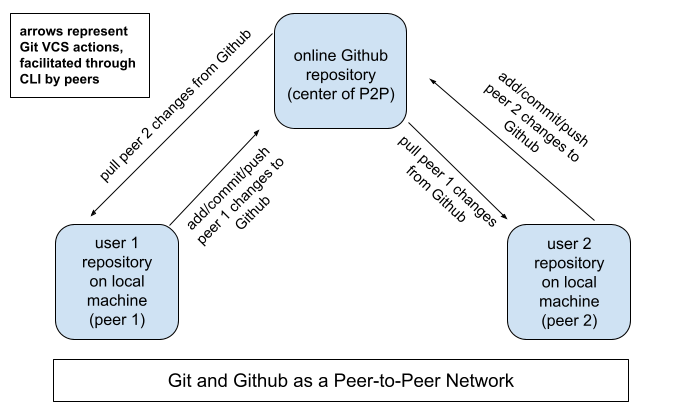
\includegraphics[width=.8\textwidth]{./images/github_p2p_flowchart.png}
\caption{"Flowchart of the P2P circulation of information from user to user on Github."}
\vspace{0in}
\end{center}
\end{figure}
In the flowchart above, the way Git and Github operate as a P2P network is shown. The top of the diagram is the remote repository on Github, which acts as the centralized nature of the system, along with the established Git Flow process of add/commit/push, and lastly the pull of new changes from the remote repository. The lower nodes in the flowchart are the repositories on the local machines of the users, user 1 and user 2, which both represent the peers in the system. To be a peer in this specific system is to be the origin of changes made to the code and information added to the repositories, and facilitating the circulation of information. The sharing of information relies on the actions of the peers. Although not shown the flowchart, the peers will take the decentralized action of adding their own changes in their local repositories. Then, user 1 will use Git send their changes into circulation, carried by Git, through Github, and then to user 2, and vice versa. Through Git and Github, the peers pass information to the other peers in this network. 

Because Git acts as the connecting piece in the P2P system from the peer node to the central server which is Github, and this is how information circulates through the project in the repository and the open source software community of contributors associated with the repository, it is necessary to address what this action means in terms of how Github functions as a library. This P2P system is what characterizes the circulation of information in Github repositories, similar to the circulation of information through physical libraries, but different because this circulation is more decentralized than the physical library. Additionally, peers in the Github P2P system pull or "check out" information through Git from Github, and can also "push" or add the information back into the library system in their new changes format. This is different from checking out a book from the library which is required to be returned in it's original form. Within the Github system, unlike the physical library, it allows for the possibility of discrepancies between local versions of the repository. A contributor could pull the repository and never pull it again while it continues to change on Github. The contributor could also make changes to their local repository which are never pushed to Github. This occurs because Git as a version control system is not automatic, and the user must use it in order for the versions to be recorded on Github. A complication with this specific to Github is how the add/commit/push process can be started, but not finished. For example, the contributor could use git add and leave the process at add, or create the commit and choose not to or forget to push it to Github with git push. 


%\numberedchapter{Integration}
\chapter{Integration} 
\label{ch:integration}

\section{Interdisciplinary Glossary}

This section concerns the Interdisciplinary Glossary, a new set of terms developed to support the interdisciplinary nature between Library Science and Computer Science on both the technical and disciplinary level. This glossary is separate from the thesis glossary, but terms from the Interdisciplinary Glossary have been influenced by the thesis terminology. 

\subsection{Purpose of this Glossary}

The purpose of defining this new terminology is to allow for more specific discussion of the interdisciplinary relationship between library science and computer science. This includes more concisely applying multiple similar, yet different ideas from library science to Github, and addressing the Peer-to-Peer qualities of Github and how these intersect with the idea of circulation in libraries. It is necessary for these terms to exist to better solidify the interdisciplinary relationship between computer science and library science in a practical sense, and bridge the gap between larger-scale conceptual discussion and practical application. Some of the terms already exist in library science and have been re-defined for interdisciplinary conversation, merging the meaning for the term for both disciplines or merging the library science meaning with a new computer science meaning and vice versa. 

In order to validate the meaning and establish the practical use of the interdisciplinary terminology, this terminology will be applied throughout the pandas case study in discussion. A major part of the interdisciplinary terminology is the establishment of the Github Circulation Network and the associated terminology. This is the name given for how information circulates on Github, which as discussed in the Concepts chapter, occurs on a P2P network. The following subsection will illustrate and break down the Github Circulation Network using the new Interdisciplinary Glossary terms which apply to it. 

\subsection{Github Circulation Network}

\begin{figure}[hbt!]
\begin{center}
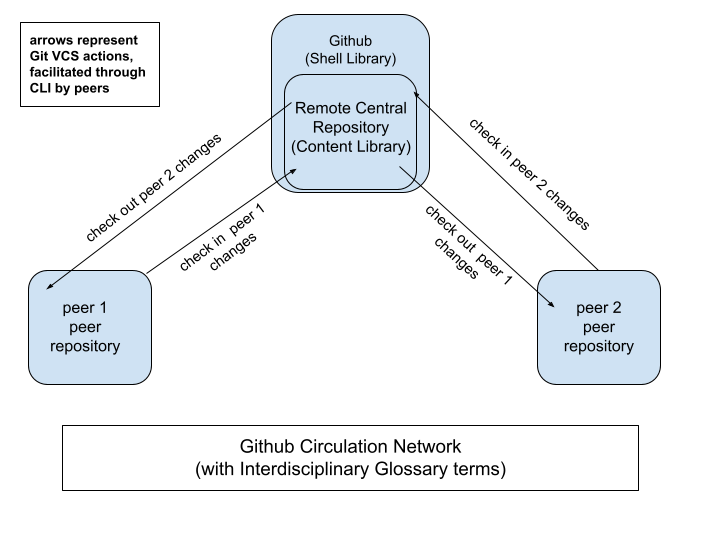
\includegraphics[width=.8\textwidth]{./images/gcn_flowchart.png}
\caption{"Illustrating the P2P GCN using interdisciplinary glossary terms."}
\vspace{0in}
\end{center}
\end{figure}

The above flowchart, similar to that in the P2P section of the Concepts chapter, approaches the same concept using the new Interdisciplinary Glossary terms. Here, the network is named Github Circulation Network, to reflect how this P2P system represents the circulation of information through Git and Github. The two lower nodes where the information originates are now labeled "peer repository", to reflect how the repositories on the local machines function as the endpoints of each peer node, and are therefore the peer's repository. The remote repository on Github has been renamed the "remote central repository" to reflect the position as the remote version of the repository on Github, and that it is the centralized piece of the P2P network. 

Additionally, note that the remote central repository includes the name "content library" and is held within another box labeled "shell library", which represents Github. The addition of this nested node structure has been added to represent how Github functions as a library entity. In physical library systems, there is often a central library and many branch libraries, which are bound to this central library in that library system. On Github however, individual repositories function as their own entities with their own development communities, held within the overall structure of Github as a "shell". Then, Github as a "shell library", includes the repositories which contain the projects and their associated communities, and therefore the content of the library. Because of this, the term "content library" has been assigned to repositories. Then, the content library sits within the shell rather than attached to, because it is part of the decentralized library-like system of Github.  

\subsection{The Community Code Archival Librarian}

The term "Community Code Archival Librarian" (CCAL) has been given to the the methodology of understanding who carries out the actions of the librarian defined by Gorman \cite{gorman2000values} and the SAA values \cite{rubin2016foundationslis} which apply to Github based on discussion in the Concepts chapter. The name "Community Code Archival Librarian" has been chosen to reflect the importance of written code and the overall work of the associated communities for FOSS projects. "Archival Librarian" has been chosen to reflect the the inclusion of both actions of the librarian and SAA values in this new term. In giving this term a name, it is necessary to note the difficulty in including the true scope of the materials this position works with archiving. For example, "code" and "community" do not accurately reflect the importance of documentation in software projects, although this is attempted to be included through the "community" aspect, as that documentation, all the issue discussion, project board organization, and pull request processes are all work of the collective FOSS community for each repository.

These are the actions of the CCAL: 
\begin{itemize}
    \item select\cite{gorman2000values}/selection\cite{rubin2016foundationslis}
    \item acquire \cite{gorman2000values}
    \item organize and give access \cite{gorman2000values}
    \item preserve and conserve \cite{gorman2000values}
    \item assist \cite{gorman2000values}
    \item instruct \cite{gorman2000values}
    \item access and use \cite{rubin2016foundationslis}
    \item accountability \cite{rubin2016foundationslis}
    \item advocacy \cite{rubin2016foundationslis}
    \item diversity \cite{rubin2016foundationslis}
    \item history and memory \cite{rubin2016foundationslis}
    \item preservation \cite{rubin2016foundationslis}
    \item professionalism \cite{rubin2016foundationslis}
    \item service \cite{rubin2016foundationslis}
    \item social responsibility \cite{rubin2016foundationslis}
    \item administer and manage 
\end{itemize}

\section{Integration of Concepts with Github}

In this section, the concepts discussed in the previous chapter will be applied to the Github repository for the pandas project to understand how this active repository and software community function as a library, and where the actions of the librarian are carried out in this specific community. Pandas has been chosen because this is a popular repository on Github with a community that seeks to fully utilize the different components of the repository structure that have been discussed in the Concepts chapter. This application of concepts to pandas will function as a case study for Github functioning as a library archive and the application of interdisciplinary glossary terms in a practical environment. 

\subsection{pandas Repository Overview}

The pandas repository is the main repository is the main repository under the pandas-dev organization on Github, According to the About section in the pandas repository, this project is a "Flexible and powerful data analysis / manipulation library for Python, providing labeled data structures similar to R data.frame objects, statistical functions, and much more"\cite{pandasrepo}. About 90 percent of the project is written in Python according to the languages bar in the Code section of the repository\cite{pandasrepo}. 

For the most rational and organized approach to discussing the application of Library Science concepts, the discussion will follow the tabs in the repository from left to right and break down the repository contents from those within that tab, beginning with the Code tab. 

\subsection{Repository Template}

The repository template refers to a blank Github repository in the state when it is first created. At this time, it includes all of the tabs mentioned, but lacks the information within and a README. This baseline repository set up to organize information by tabs and sectioned off within each page reflects Gorman's value of Rationalism by approaching the organization of information in a repository from a technical perspective which is "independent of emotions, faith, and the senses" as Gorman defines Rationalism \cite{gorman2000values}. Encapsulating information in the tab structure allows contributors to quickly switch between different parts of the repository and maintain focus on one area at a time as well. The template including the Code page with the most recent commit, repository file system, and centering the major source of documentation that is the README, which also may link the CONTRIBUTING.md file, also reflection Rubin's value of Truth and Search for Truth by making available information \cite{rubin2016foundationslis}.

\subsection{Code}

The Code tab, being the first tab to the left of all which make up the repository, essentially functions as the home page. It includes all the branches of the repository, all the commits and displays the most recent commit name and the username of the individual who pushed the commit to Github or merged the pull request, the folder structure of the repository, the README, and a sidebar which includes an about section, the license, releases, and the bar which represents the breakdown of programming languages used in the repository. 

\subsubsection{Branches}

\begin{figure}[hbt!]
\begin{center}
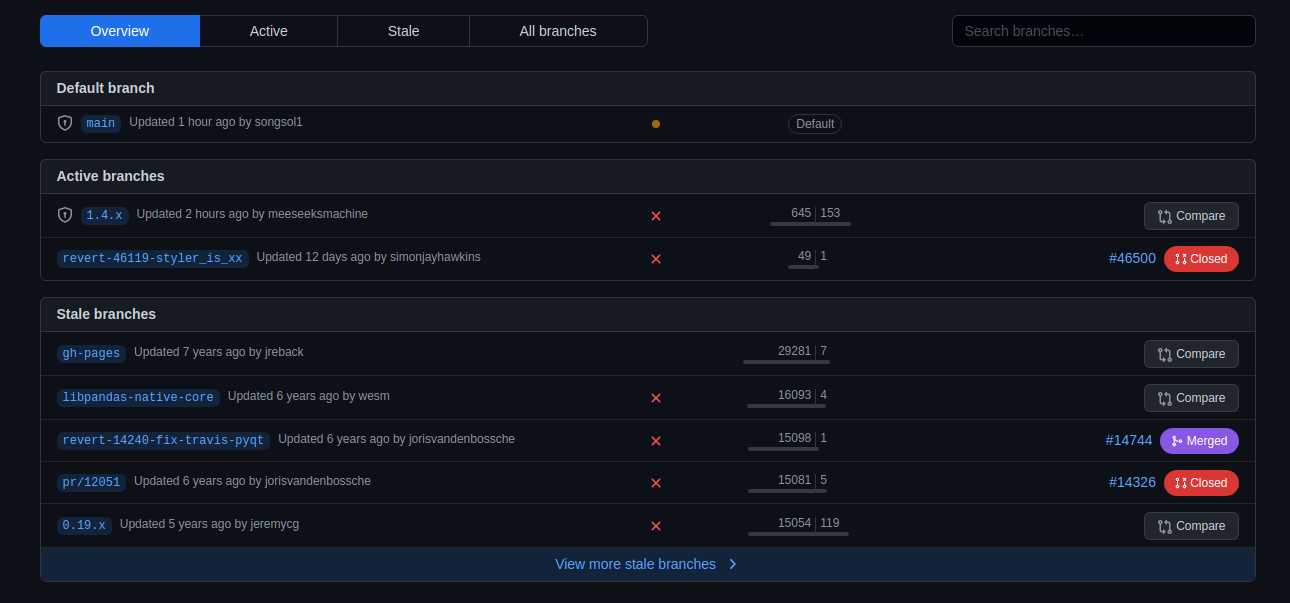
\includegraphics[width=.8\textwidth]{./images/branches.png}
\caption{"Branch page within the Code tab"}
\vspace{0in}
\end{center}
\end{figure}

Considering the use of branches is important to this research because of how the branches compare to those of a physical library system. In a physical library system, there is the central branch and other satellite branches, where information can circulate between branches, and some branches contain information which others do not. Typically, the central branch holds the largest collection. 

Branches are used as part of Git Flow to allow for collaboration of the repository without merge conflicts. A new branch is essentially another copy of only the file system in the repository. This is the file system which is brought to the local machine when "git clone" is used, and does not include the full repository structure on Github, as it lacks pieces such as the Issue Tracker and Pull Requests. This differs from a fork of a repository, which is a copy of the whole repository on Github, including all of the tabs such as the Issue Tracker and Pull Requests. 

Contributors can add new information, change existing information, and delete information in a branch and it remains local to that branch. This is then pushed to the remote branch on Github. The difference in information between a satellite branch and the main branch reflects the difference in information which occurs between branches in the circulation of information in the physical library system. In difference between the two is that the physical library allows for circulation of materials from the central branch to the satellite branch, whereas it is not possible to merge the main branch into a satellite branch on Github, it is only possible to create a pull request that merges changes from the satellite branch into the main branch. Github tracks the difference in versions in terms of commits for each branch of the repository. For example in pandas, there is a bar above the most recent commit in the 1.4.x branch which notes "This branch is x commits ahead, x commits behind main"\cite{pandasrepo}. This is an example of how Git as a version control system takes on actions of the CCAL to record the history of changes in the repository. 

\subsubsection{Commits}

The most recent commit bar includes a link at the end, which appears as a clock followed by the number of commits in the repository, excluding commits that have been squashed into one. The commits are grouped by day. The commits function as links to the diff page, which shows a side by side comparison for every file changes, with the left side showing deletions and the right side showing additions. This diff page functions as a representation of the actions that occur at the peer end of the Github Circulation Network, by showing information which has been removed from the current version of the project and therefore removed from further circulation. It is important to note that this removal is only to some extent, as it is not possible to remove this from previously existing forks that have not been merged or commit-absent copies. Commit "Fix CI" in the pandas repository will be considered as an example for understanding the Github Circulation Network in a practical application. 

\begin{figure}[hbt!]
\begin{center}
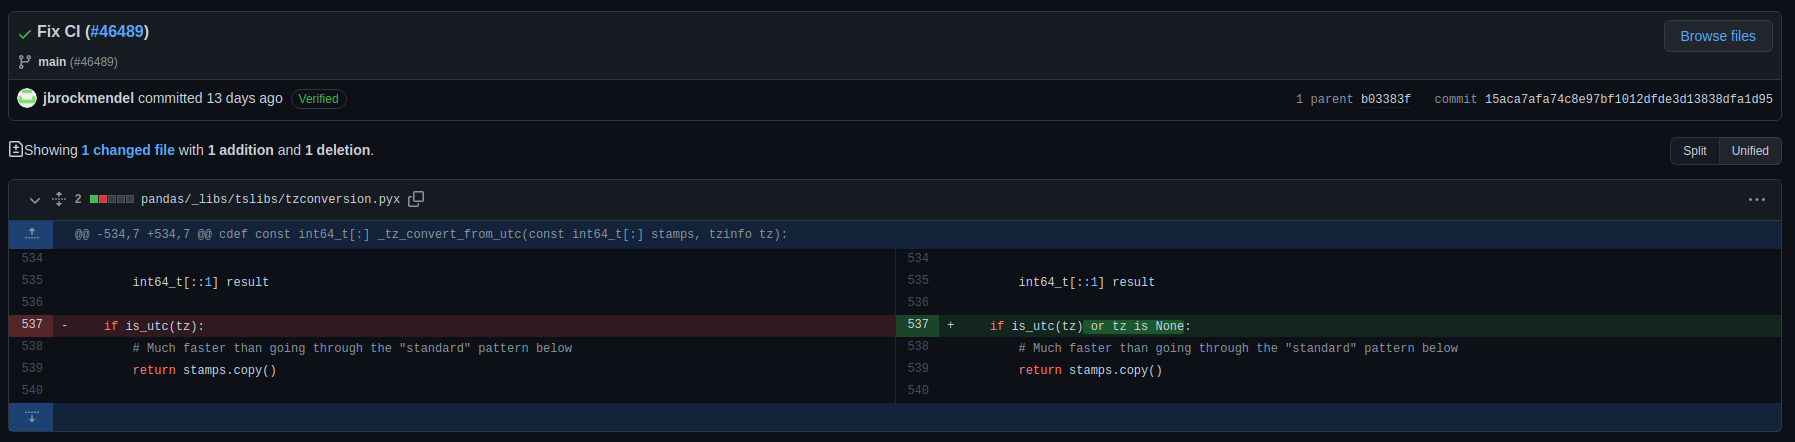
\includegraphics[width=.8\textwidth]{./images/fix_CI_diff.png}
\caption{"Fix CI commit diff page to view changes made"}
\vspace{0in}
\end{center}
\end{figure}

Commit "Fix CI" , pushed to Github by jbrockmendel, includes a change in an if statement they made on line 537 of the file tzconversion.pyx, as shown on the diff page for this commit, which adds to the end of the existing if statement "or .tz is None" \cite{pandasrepo}. As a result of this change in the main branch of the repository, local versions of the repository which have not checked out this new version have now become commit-absent copies of the repository because they are behind in the commit history. As previously stated, this diff page represents the change which was made in the peer repository of the Github Circulation Network. Then, this addition went through the add/commit/push process using Git, which shared this information to the remote central repository on Github. Now that the change in this if statement is in the remote central repository, other peers in this network are able to check out the new version of the repository to their peer repository, completing the full peer-to-peer process of the Github Circulation Network. 

\subsubsection{Releases and Packages}

Similar to commits, releases and packages are a way in which Github functions as a version control system. According to the Packages section of the pandas repository, there are no packages available, so this section will instead focus on releases since this is utilized by pandas \cite{pandasrepo}. Each new release functions as an update for the pandas tool, facilitated through the Git command "tag" by maintainers of the repository \cite{gitdocs}. On the Release page, it is possible to choose between seeing full releases or the list of tags, which are the version of the releases. Each release on the Release page still includes the tag number. For example, the most recent release was facilitated by simonjayhawkins and the tag for the release was 1.4.1 \cite{pandasrepo}. The preservation of the code and documentation in this release reflects Rubin's value of The Public Good, characterized by Rubin as "preserving the cultural record" \cite{rubin2016foundationslis}. This is because each release includes the source code at the time of that release, which is preserved in that state even when future releases are made. The source code qualifies as cultural record because it is a result of the collaboration of the pandas community, and includes the contributions of many people. There may be contributions which are altered in future releases, but remain intact from how the original author created them in the 1.4.1 release. 

Additionally, multiple actions of the CCAL have been carried out for releases. As a maintainer making releases, simonjayhawkins has carried out the action of Select by choosing the point at which the release would be made and no further changes would be included in the 1.4.1 release \cite{gorman2000values}\cite{rubin2016foundationslis}. The action of Organize and Give Access was taken, because there are CLI commands given along with the release to download and upgrade pandas to the new version \cite{gorman2000values}. These commands may also fall under Instruct since the commands could be considered instruction for download \cite{gorman2000values}. Lastly, the record of the release would qualify as an act of preservation for preserving the project code in the moment of the release without accounting for future changes made after the release date, which is Feburay 12th, 2020 for 1.4.1 \cite{rubin2016foundationslis}\cite{pandasrepo}.

\begin{figure}[hbt!]
\begin{center}
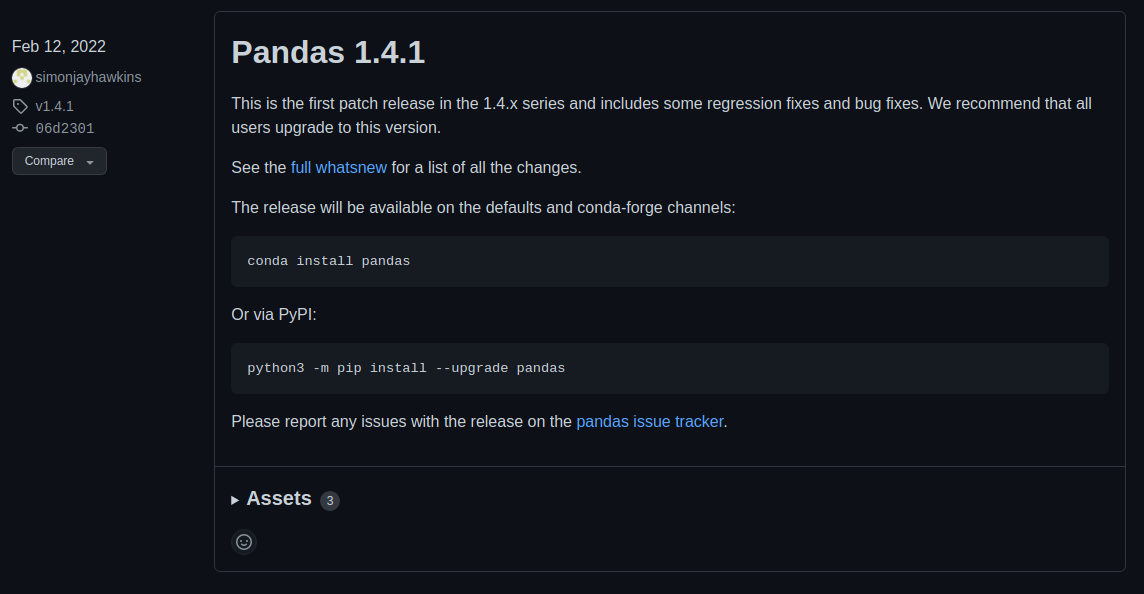
\includegraphics[width=.8\textwidth]{./images/releases.png}
\caption{"Release 1.4.1"}
\vspace{0in}
\end{center}
\end{figure}

\subsubsection{README}

An interesting quality of the README is that it is not immediately part of the repository template. Rather, the template prompts the repository owner to create a README, and READMEs are considered to be best practice for using Github. The README being a markdown file includes crucial information about the project and contributing to it. The README itself through the organization of information using headers and lists available in Markdown reflects Gorman's value of Rationalism \cite{gorman2000values}. In the pandas repository, the README includes several sections: buttons with key information (such as version number, license, and code testing coverage), What is it, Main Features, Where to get it, Dependencies, Installation from sources, License, Documentation, Background, Getting Help, Discussion and Development, and Contributing to pandas\cite{pandasrepo}. 


The README being the major source of documentation in the repository also reflects Gorman's value of Literacy and Learning \cite{gorman2000values}. This is a less specific application because the users and contributors must seek out the information in the README, although they can certainly ask questions to the project's community through the issue tracker. The README also takes on Gorman's Librarian action of Assist Library Users \cite{gorman2000values}, which also falls under the actions of the CCAL as defined in the Interdisciplinary Glossary. In this case, it could be considered either Github or the contributors who ultimately carry out this action because Github holds the README file but this is not included in the repository template, and must be organized and filled with information by the contributors and maintainers. In pandas, the Assist would be reflected through the contributing guidelines in the pandas documentation, which is linked in the README file but hosted on a separate website specifically for documentation. The inclusion of documentation for contributing reflects the CCAL action of preservation \cite{rubin2016foundationslis}. 

\subsection{Issues}

The Issue Tracker can be sorted between both open and closed issues, keeping record of all prior issues and the comments within even once the issue is closed. It is possible to filter through the issues by author, label, projects, milestones, and the assignee. There are labels given by the repository template, but it is possible to add new labels or more specific organization. Pandas had utilized this feature, adding labels such as Admin for "administrative tasks", CI for "continuous integration", and Linux for "Linux OS" within the total of 130 different labels \cite{pandasrepo}. The use of many labels to organize the issues might be considered classification, which Gorman includes in defining the action of Organize and Give Access \cite{gorman2000values}. The labels also help the contributors and maintainers better access specific information by searching for labels. By applying the labels to issues contributors and maintainers are carrying out actions of the CCAL, as Organize and Give Access is considered one of those actions.

\subsubsection{Open Issues}

Issue 46485 BUG: isin() give incorrect results for uint64 columns will be considered as an example of an open issue, because it includes discussion through comments between two contributors \cite{pandasrepo}. The issue was opened by AlexSingle, who carried out the actions of a CCAL as discussed above by adding the labels "Bug" and "Needs Triage" to the issue after it was created \cite{pandasrepo}. Contributor Saxeman commented on the issue to claim it, and was automatically assigned to the issue by the github-actions bot \cite{pandasrepo}. The github-actions bot in this instance acts as the CCAL through the action of Organize and Give Access by "maintaining online systems" \cite{gorman2000values}. 

\begin{figure}[hbt!]
\begin{center}
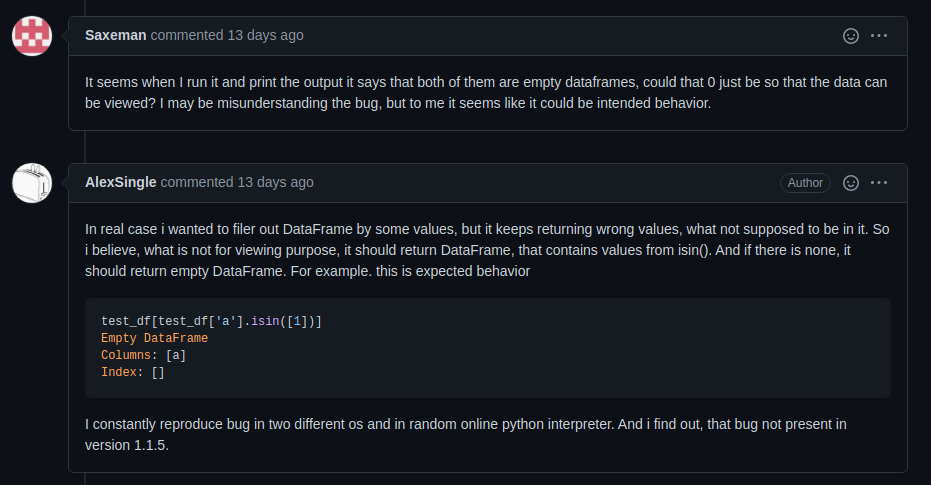
\includegraphics[width=.8\textwidth]{./images/issue_discussion.png}
\caption{"Discussion in Issue Tracker on Issue 46485"}
\vspace{0in}
\end{center}
\end{figure}

Over a few comments on this issue, Saxeman asks a question to AlexSingle to better understand the bug and another follow up question, which AlexSingle answers with code examples \cite{pandasrepo}. The documentation of this conversation in the issue tracker reflects Github carrying out the actions of the CCAL through Accountability, by keeping record of the conversation which will remain recorded even once the issue is closed \cite{rubin2016foundationslis}. Additionally, Tolerance is present here through the discussion between the two contributors with the goal of understanding how the bug worked in order to find a solution \cite{rubin2016foundationslis}. In this instance AlexSingle responding with guidance for understanding the bug is an instance of the Assist action \cite{gorman2000values}. 

\begin{figure}[hbt!]
\begin{center}
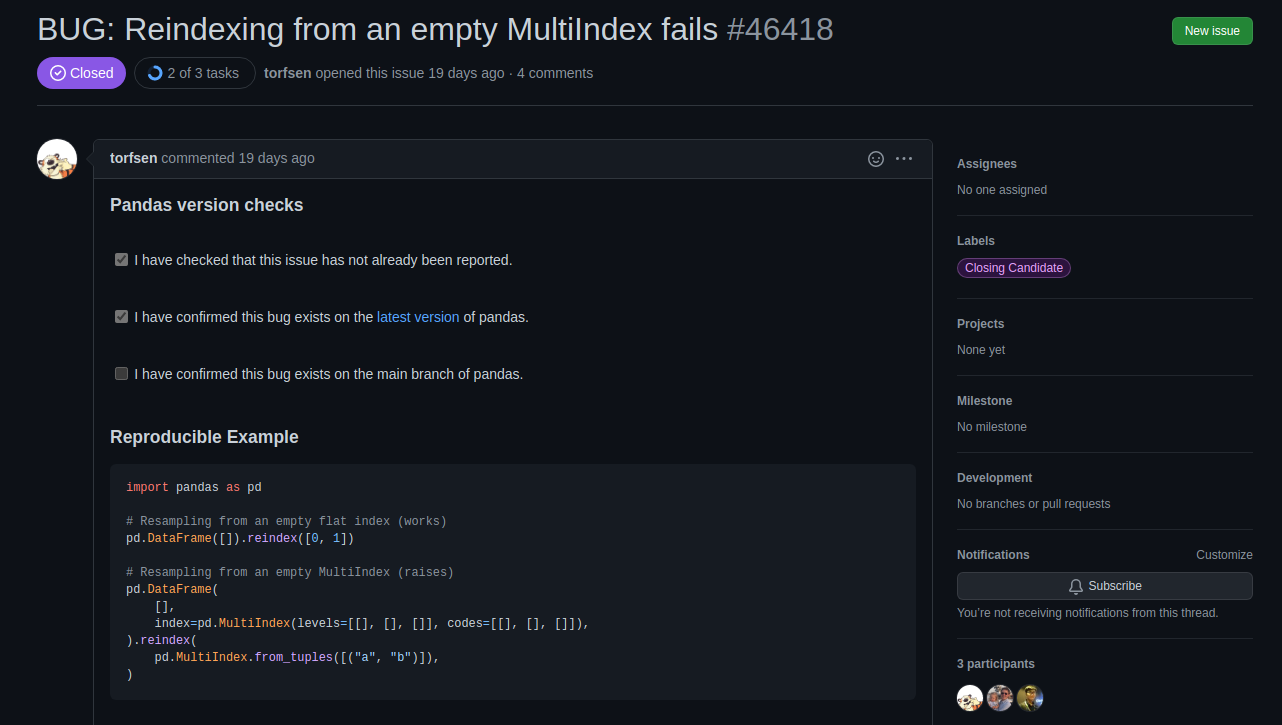
\includegraphics[width=.8\textwidth]{./images/closed_issue.png}
\caption{"Closed Issue 46418"}
\vspace{0in}
\end{center}
\end{figure}

\subsubsection{Closed Issues}

An an example of a Closed Issue, Issue 46418 will be considered, which is titled BUG: Reindexing from an empty MultiIndex fails \cite{pandasrepo}. By Github keeping record of all issues once they are closed, the platform is taking on qualities of the library and actions of the CCAL. First, Github is engaging in the core value of Stewardship by keeping record of the full conversation, which may be considered "preserving the human record" since this conversation is record of the open source community interactions \cite{gorman2000values}. Additionally Archivist values of history and memory, as well as preservation are present as the closed issue remains preserved by Github and it becomes part of the history of the community associated with the pandas repository \cite{rubin2016foundationslis}.

\subsection{Pull Requests}

The main page of the Pull Request tab appears in exactly the same format as the Issues tab, including the pages of open and closed issues, the drop down tabs to sort by author and so on, and the same 130 labels available to organize issues \cite{pandasrepo}. Open PRs have not been merged or closed and are indicated by the green icon. Closed PRs are usually merged, indicated by the purple icon, but may remain unmerged, indicated by the red icon. Because of the similarity between the Issues and Pull Request as community discussion spaces local to Github and their overall format, both will share actions of the CCAL and qualities of libraries that apply. 

In an open source project like pandas where commits must be merged into the project in order for the commits to be part of the main branch and new releases (unless further changes are made to that work), pull requests function as the last step of the Github Circulation Network. Although the contributions of all contributors remain recorded in branches in the repository and forks on Github, this likely is not being used by other contributors and users like the main pandas project would be. 

The major difference between pull requests and issues is that pull requests function as part of the Github Circulation Network, while issues do not. The pull request, as mentioned, is the final step in the Github Circulation Network for checking in new information in FOSS projects because it is the addition of the commits into the main branch of the repository, where those changes can be pulled to peer repositories, completing the network. There may also be a difference in how Selection occurs at the PR stage, as this occurs after development has occurred, where discussion in the Issue Tracker occurs before or during development \cite{gorman2000values}\cite{rubin2016foundationslis}. 

\subsubsection{Open Pull Request}

\begin{figure}[hbt!]
\begin{center}
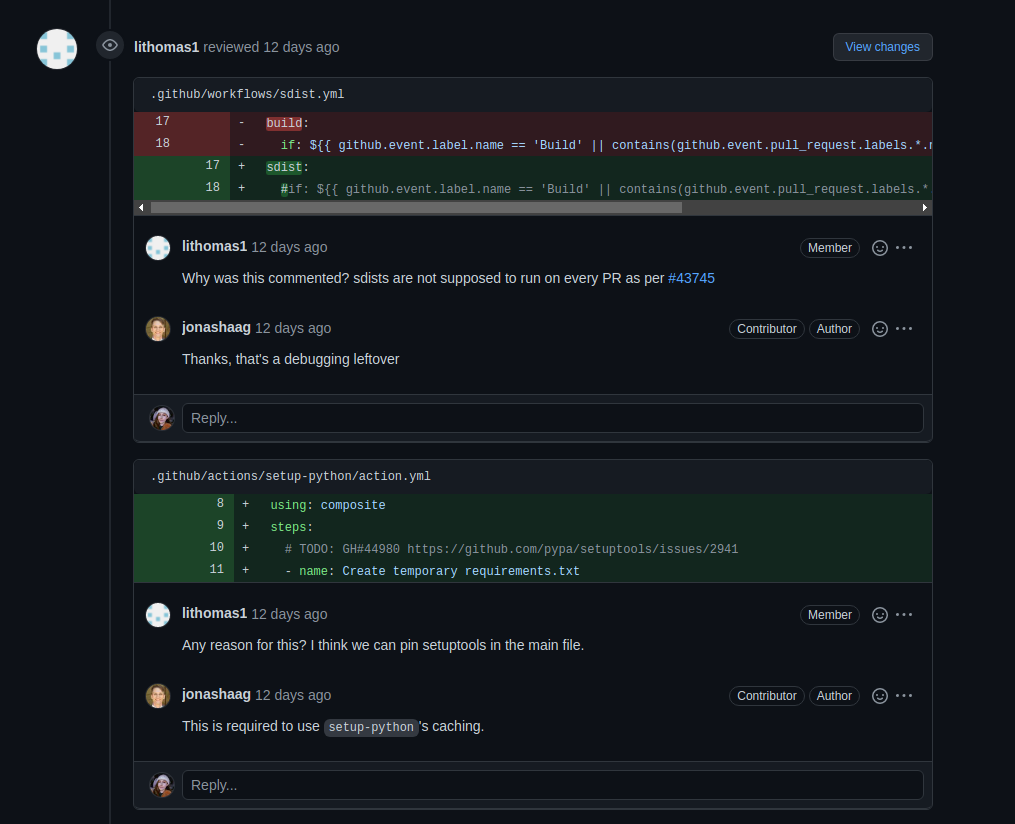
\includegraphics[width=.8\textwidth]{./images/pr_review.png}
\caption{"PR Review by maintainer on PR 46493 Refactor CI"}
\vspace{0in}
\end{center}
\end{figure}

Pull Request 46493 Refactor CI will be considered as an example of an open pull request due to the documentation of a conversation on what changes should be included in the final merge \cite{pandasrepo}. Through the discussion in the comments of the PR, the contributors are deciding what will and will not be included in the potential merge. By submitting a pull request, contributor jonashaag is engaging in Gorman's value of Intellectual Freedom to some extent, by showing their commits which they wish to be part of the project \cite{gorman2000values}. However, whether these commits are merged into the project is ultimately the choice of the maintainers, and changes may be requested to the existing work before it is merged. Reviewer lithomas1, acting as the maintainer by reviewing jonashaag's PR, added two comments with changes/questions. By reviewing this PR, lithomas1 is acting in service for the development community of pandas, which is an example of Rubin's value of Service, "underlying the value of service is the belief in the betterment of the individual and the community as a whole" \cite{rubin2016foundationslis}. This action of reviewing the pull request also qualifies as an action of the CCAL through the archivist action of service \cite{rubin2016foundationslis}. Because the conversation through open pull requests determined what is and is not merged into the project, jonashaag and lithomas1 are both carrying out the actions of the CCAL, specifically Gorman's library action of Select and the archivist action of selection \cite{rubin2016foundationslis} \cite{gorman2000values}. After lithomas1's review, other maintainers join the conversation of the pull request

\subsubsection{Closed Pull Requests}

Similar to how Github handles closed issues, the full record of the pull request including comments is preserved on Github under the closed PR section of the Pull Request tab. For PRs, the state of the pull request at the time of closing it is also recorded, whether it was merged or closed. Closed PRs, both merged and closed without merging, will be studied. 

For the PR closed without merging, PR 46531 change default value (for index) of func named to\_cvs created by a5chin will be studied \cite{pandasrepo}. In the comments of this issue, maintainer jreback is the reviewer of the PR and engages in discussion about there not being an issue associated with the pull request, which is required for the change a5chin would like to merge into the project \cite{pandasrepo}. Another maintainer, mroeschke, comments on the PR confirming that there needs to be community discussion through an issue, and notes that they will close the PR until that discussion occurs \cite{pandasrepo}. In this instance, the maintainers are upholding the CCAL value of Professionalism by requiring the contributor to follow the issue tracker discussion step of the contributing process \cite{rubin2016foundationslis}. Similar to how Github preserves the conversation with issues, the value of Stewardship applies to how Gitub keeps record of the umerged PR, which shows the value of recording the community interaction and all contribution, even if that contribution is incomplete and not included in the project \cite{gorman2000values}. However, in the case of PR 46531, Github's ability to carry out Stewardship to the full extent of documenting the commits as part of this PR is complicated by a5chin's choice to completely delete the branch holding their work \cite{pandasrepo}. This could negatively impact the community by deleting work which could have been merged if an issue had been created for community discussion, as requested by the maintainers. Even if the work was abandoned by a5chin, maintainers or other contributors could have picked up the work and continued with it. Because Github has preserved this closed PR, it may still be possible to salvage the available information about the work from the comments. Evidently, Github has acted as the CCAL here through the values of history and memory, and preservation \cite{rubin2016foundationslis}. It is possible to see through the record of conversation and the last action notes on the PR of a5chin deleting the branch how recorded code can be lost, and understand the potential consequences for the community when a contributor withdraws their work, which qualifies this as valuing history and memory \cite{rubin2016foundationslis}.

\begin{figure}[hbt!]
\begin{center}
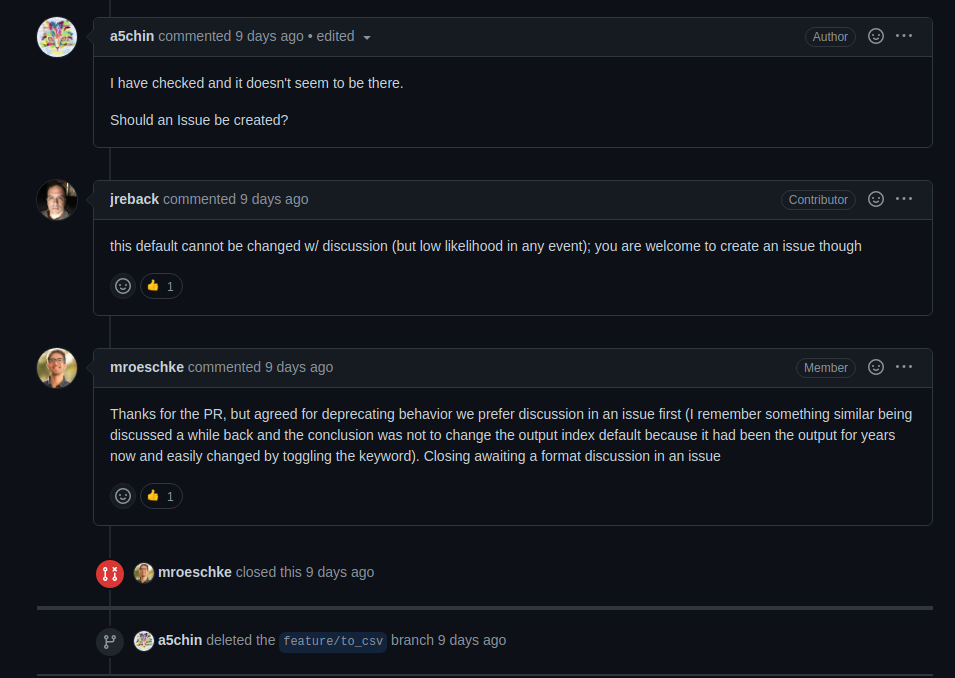
\includegraphics[width=.8\textwidth]{./images/closed_no_merge.png}
\caption{"PR closed without merging"}
\vspace{0in}
\end{center}
\end{figure}

\begin{figure}[hbt!]
\begin{center}
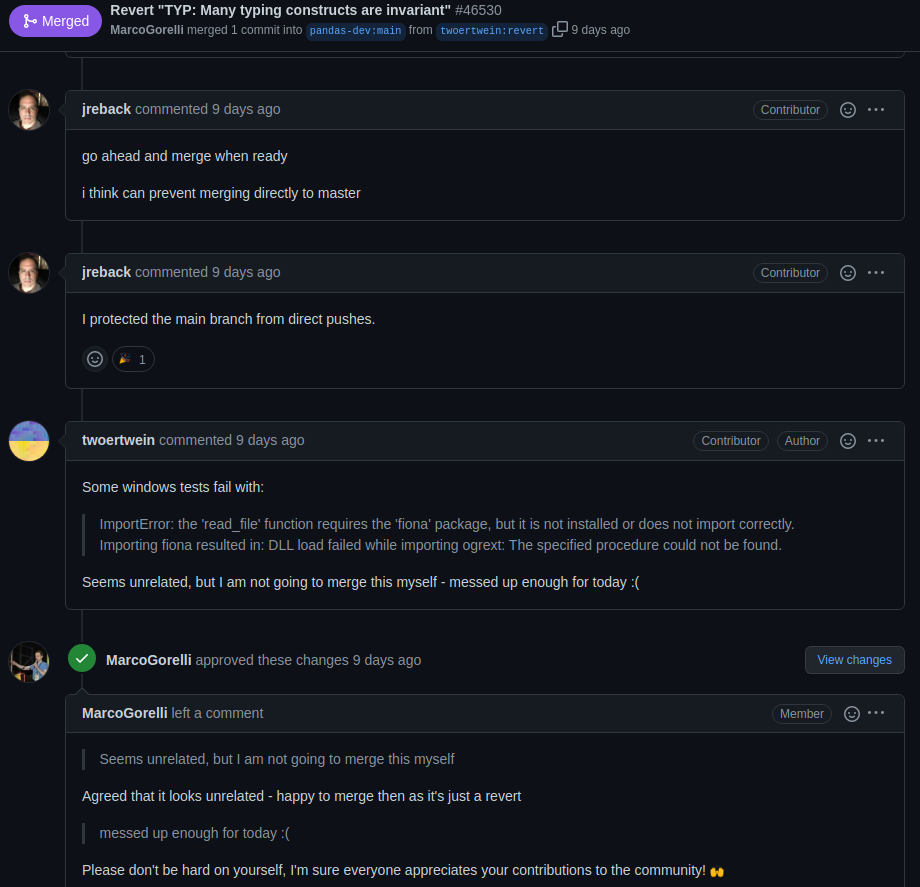
\includegraphics[width=.8\textwidth]{./images/merged_pr.png}
\caption{"Discussion between contributor and maintainers on PR closed due to merge"}
\vspace{0in}
\end{center}
\end{figure}

For the pull request which has been closed due to a merge, PR 46530 Revert "TYP: Many typing constructs are invariant" will be studied \cite{pandasrepo}. According to the PR title and comments from twoertwein, the contributor who opened the PR, this PR reverts to a prior version of pandas because twoertwein pushed to the main branch rather than their own \cite{pandasrepo}. Two maintainers, jreback and MarcoGorelli, review the changes and stop other commits from being able to be pushed to main \cite{pandasrepo}. MarcoGorelli specifically addresses twoertwein's concerns about completing the merge for this PR successfully, comments with reassurace about their work being valued for the project, then completes the merge for the PR \cite{pandasrepo}. In this PR, MarcoGorelli and jreback are upholding the value of service for the pandas community by reviewing this PR, and MarcoGorelli by giving encouragement to a member of the community and therefore helping create a positive community space even when a contributor makes the mistake of pushing to the wrong branch \cite{pandasrepo}\cite{gorman2000values}\cite{rubin2016foundationslis}. In this instance, jreback as a maintainer carries out the CCAL action of organize and give access by restricting push access to the main branch of the pandas repository \cite{gorman2000values}. The same actions of the CCAL which applied to the closed unmerged pull request apply to this PR, with the additional understanding that Github carries out the actions of Social Responsibility and Accountability through preserving the comments of the pull request, which are just one piece of the interactions in the pandas community and can be used to verify the actions of community members \cite{rubin2016foundationslis}. By revoking the ability to push directly to the main branch, maintainers jreback and MarcoGorelli are carrying out the CCAL action of access and use \cite{rubin2016foundationslis}, in addition to administer and manage\cite{gorman2000values}. 

\subsection{Actions}

In a Github repository, the Actions tab shows a list of all the bots which operate within that repository. When the name of the bot in clicked on, it shows a link to the .yml file which controls the actions of the bot and the list of contributors who built it. Underneath this link is a list of all the instances where the bot was run, which are called workflows, including the total number of workflows for the full history of the bot. These records of each workflow run include the contributor whose action caused the bot to run a workflow, what the status of the workflow is, and the time it lasted \cite{pandasrepo}.

\subsubsection{Bots in Maintaining Repositories}

\begin{figure}[hbt!]
\begin{center}
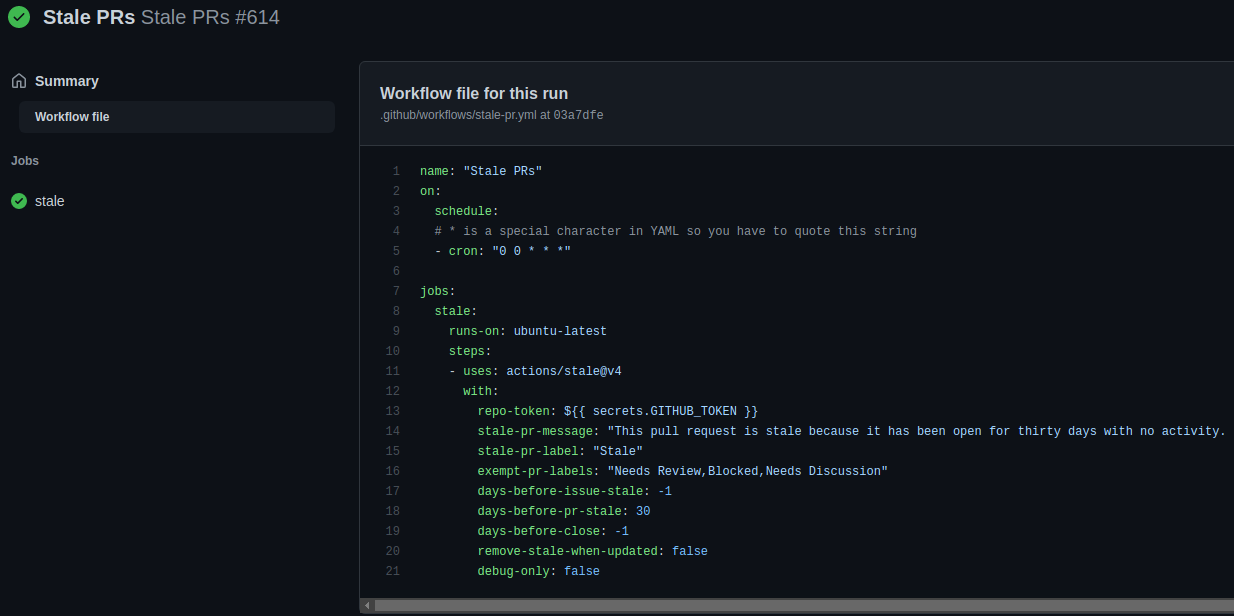
\includegraphics[width=.8\textwidth]{./images/actions_pr_bot.png}
\caption{"Code file for the Stale PR bot."}
\vspace{0in}
\end{center}
\end{figure}

Considering the Stale PRs bot, the last workflow was run according to the schedule it is based on and this workflow run was a success, and this workflow lasted 53 minutes \cite{pandasrepo}. Looking at stale-pr.yml, it is shown that two maintainers built this file rather than the bot being part of Github, which qualifies as the maintainers carrying out the CCAL action of service by creating a bot that serves the community \cite{gorman2000values} \cite{rubin2016foundationslis}. Because the service to the project community in maintaining stale PRs is carried out by the bot, the action of service applies to the Stale PRs bot as well \cite{gorman2000values} \cite{rubin2016foundationslis}. In building the bot, the maintainers are ensuring that the CCAL actions organize and give access, preserve and conserve, and preservation are carried out in the Pull Requests by the bot. Organize and give access applies because the PRs are closed after 30 days of no activity and recorded so that they may be opened again in the future, which preserves them but helps keep the open PRs limited to active conversation and activity \cite{gorman2000values} \cite{rubin2016foundationslis} \cite{pandasrepo}. Lastly, the value of Stewardship applies to the bot's actions of closing the PR and to Github's practice of recording closed PRs because the PRs are preserved in the closed state rather than being deleted \cite{gorman2000values}. 

\subsection{Projects}

\begin{figure}[hbt!]
\begin{center}
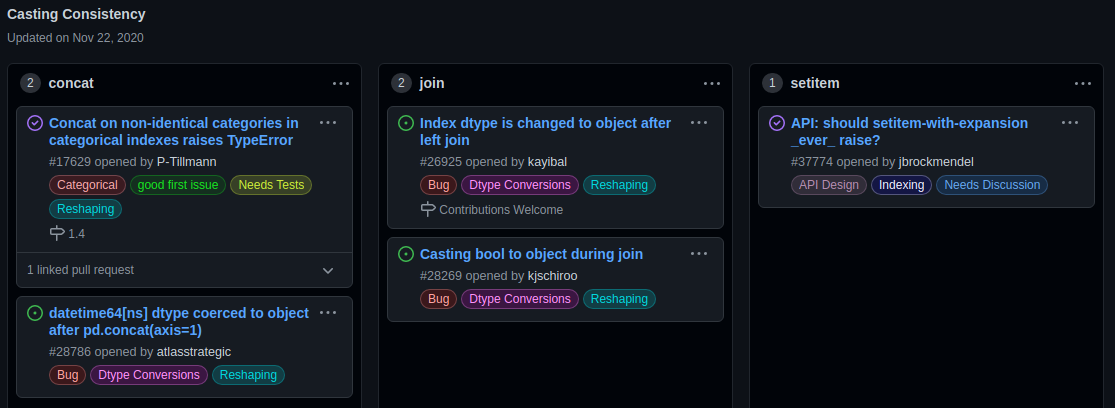
\includegraphics[width=.8\textwidth]{./images/project_board.png}
\caption{"Active project board in pandas."}
\vspace{0in}
\end{center}
\end{figure}

The Projects tab in the repository template is initially blank, allowing for maintainers and the community to sort issues into categories to better track the completion of a project and understand what needs to be done in what area of the project \cite{pandasrepo}. This is a space that can be used by both maintainers and contributors, as it is available to the whole community in pandas. The in-progress project Casting Consistency will be studied as an example of a project in pandas \cite{pandasrepo}. There are three columns, labeled from left to right as concat, join, then setitem \cite{pandasrepo}. Each include issues as the content of the columns, which shows the name of the issue and the tags given to the issue, which is show in a sidebar view when the title is clicked \cite{pandasrepo}. The overall structure given by Github to categorize issues reflects Gorman's value of Rationalism, shown here through the discrete, technical organization that the contributors and maintainers of pandas have chosen to use for the Casting Consistency project \cite{gorman2000values} \cite{pandasrepo}. The content of issue within the category directly applies to the title of the category. For example, the first of the two issues in the concat column is titled "Concat on non-indentical categories in categorical indexes raises TypeError" \cite{pandasrepo}. Because the projects tab is more about organization for the project community than recording information, the application of Library Science concepts is limited to Rationalism in the Projects tab. 

\subsection{Wiki}

The Wiki tab functions as a collection of links to different resources and documentation for the pandas community \cite{pandasrepo}. The main page of the Wiki includes a main section with headers: External Links (includes Docs and API reference), Reference, For Documentation Authors, For Developers (noted as being moved soon, with a link to "complete documentation"), and For Maintainers \cite{pandasrepo}. There is also a sidebar with more information for maintainers and developers, under a drop down menu of all 29 pages of the Wiki \cite{pandasrepo}. The Wiki for pandas as a whole being a rich source of documentation for understanding and contributing to the project and on Github in general qualifies the Wiki as an example of Literacy and Learning \cite{gorman2000values}. There is the complication here of the user or the contributor needing to actively seek out this information, but this process is made easier by the Wiki holding this information, and being organized into pages, including a main page with sections of information \cite{pandasrepo}. The Truth and Search for truth applies in this instance as well, because of how the Wiki more easily makes available information to those who are seeking it \cite{rubin2016foundationslis}. The Wiki also functions as the CCAL through holding information that assists and instructs both users and contributors, and professionalism through providing access to the information that guides the actions of contributors and maintainers, such as the contributing guidelines \cite{gorman2000values} \cite{rubin2016foundationslis} \cite{pandasrepo}. More specifically, the information in the pandas Wiki which by being included qualifies this as assist and instruct Using Git under the For Developers header, or the link to Google Summer of Code being included \cite{pandasrepo} \cite{rubin2016foundationslis}. For Maintainers, this would include guidelines for the merge and release processes \cite{pandasrepo}. By including access to this information, especially Google Summer of Code, pandas may be indirectly advocating for Coding Literacy by surfacing this resource \cite{vee2017coding}. 

\subsection{Security}

The Security tab includes both the Security Policy and any Security advisories associated with the repository, and although there are no security advisories on pandas, there is an active security policy\cite{pandasrepo}. When the security policy link is clicked, it redirects to a .gtihub.SECURITY.md file which links to the Tidelift website for reporting a vulnerability \cite{pandasrepo}. By including the ability for users, contributors, and maintainers to report vulnerabilities through Tidelift , the value of Privacy applies to the pandas repository \cite{gorman2000values}. According to the Tidelift security policy, "Tidelift acts as the security contact for many open source projects" \cite{tideliftpolicy}.

Taking a closer look at the Tidelift page for their security policy, this application takes an extra step in security for the reporter by providing a public key to encrypt the email when reporting vulnerabilities to Tidelift \cite{tideliftpolicy}. By providing the public key, this security service is giving an extra level of privacy for the reporter, again reflecting the value of Privacy \cite{gorman2000values}. 

\subsection{Insights}

\begin{figure}[hbt!]
\begin{center}
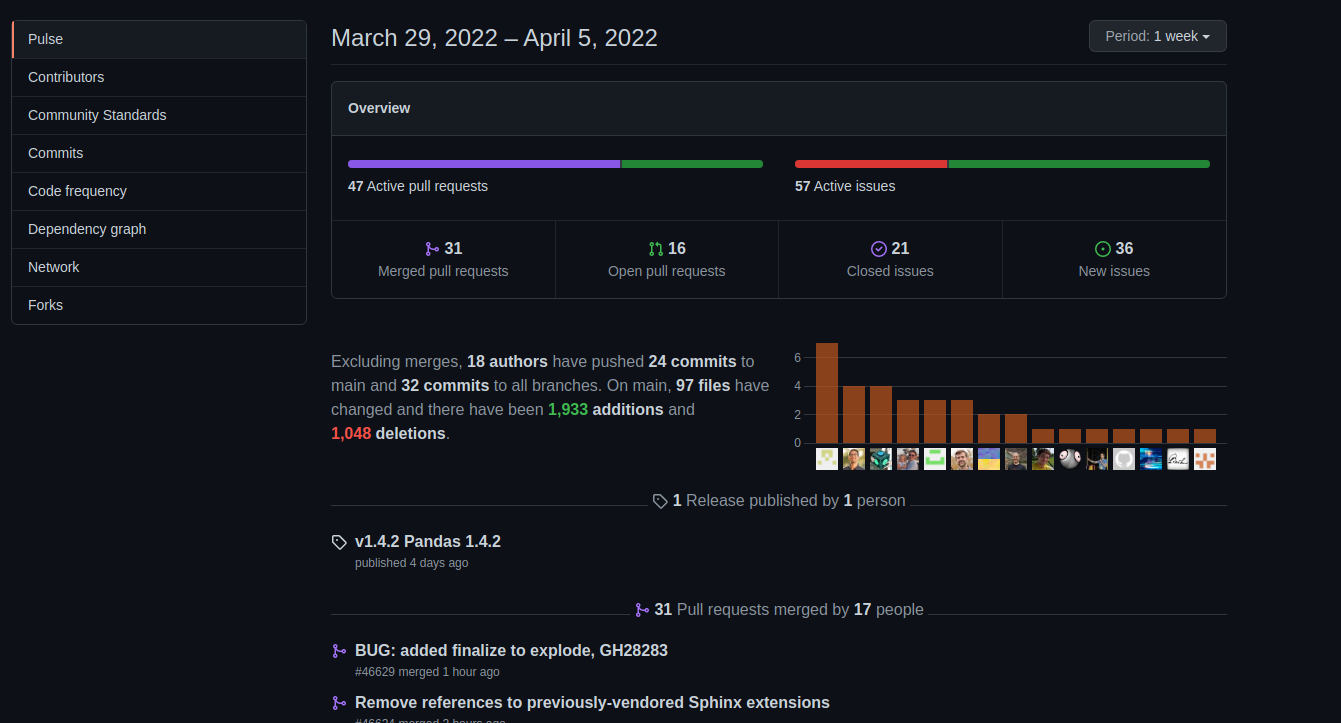
\includegraphics[width=.8\textwidth]{./images/insights.png}
\caption{"Main page of the Insights tab in pandas."}
\vspace{0in}
\end{center}
\end{figure}

Insights is the final tab in a Github repository, which includes extensive data about the repository and the community \cite{pandasrepo}. This tab is organized by Github itself, rather than being worked on by maintainers or contributors, therefore the values and actions which apply to the Insights tab apply to Github directly.  The first page, labeled "Pulse" shows graphs and lists of repository activity over a certain period of time, such as a week \cite{pandasrepo}. Through recording all contributions from all contributors in the issues and PRs, Github is engaging in the CCAL value of diversity,\cite{rubin2016foundationslis}. Additionally, values which are strongly present in the insights is preserve and conserve, as well as history and memory, because the insights tab specifically is a record of the history of the whole pandas development community \cite{rubin2016foundationslis} \cite{pandasrepo}. Graphs of commit activity for commits in the main branch are shown for each contributor, and for the repository as a whole \cite{pandasrepo}. An interesting piece of the Insights tab is the Community Standards page, which evaluates on a checklist and shown with an orange/yellow/green gradient bar the way in which the project meets best practices considered by Github \cite{pandasrepo}. This includes checks for a README, Contributing guidelines, and a License, with the only missing check being "Repository admins accept content reports" \cite{pandasrepo}. By Github including this checklist, Github is carrying out the CCAL action of accountability \cite{rubin2016foundationslis}. 

\subsection{Case Study Concluding Overview}

To summarize, this case study to analyze how Github functions as a library archive has been implemented with pandas because this a repository with high activity and an extensive community of maintainers and contributors who use Github and Git extensively, including a full range of the functions allowed by the repository. In the pandas repository, the following values of libraries and library and information science applied: 

\begin{itemize}
  \item Rationalism \cite{gorman2000values}
  \item Literacy and Learning \cite{gorman2000values}
  \item The Public Good \cite{rubin2016foundationslis}
  \item Tolerance \cite{rubin2016foundationslis}
  \item Stewardship \cite{gorman2000values}
  \item Intellectual Freedom \cite{gorman2000values}
  \item Service \cite{gorman2000values} \cite{rubin2016foundationslis}
  \item Truth and Search for Truth \cite{rubin2016foundationslis}
  \item Privacy \cite{gorman2000values}
\end{itemize}


The following CCAL actions applied to Github and the community: 

\begin{itemize}
  \item Select \cite{gorman2000values} \cite{rubin2016foundationslis}
  \item Organize and Give Access \cite{gorman2000values}
  \item Access and Use \cite{rubin2016foundationslis}
  \item Instruct \cite{gorman2000values}
  \item Assist \cite{gorman2000values}
  \item Preservation/Preserve and Conserve  \cite{rubin2016foundationslis} \cite{gorman2000values}
  \item Accountability \cite{rubin2016foundationslis}
  \item History and Memory \cite{rubin2016foundationslis}
  \item Service \cite{rubin2016foundationslis}
  \item Select/Selection \cite{gorman2000values} \cite{rubin2016foundationslis}
  \item Professionalism \cite{rubin2016foundationslis}
  \item Social Responsibility \cite{rubin2016foundationslis}
  \item Diversity \cite{rubin2016foundationslis}
  \item Administer and Manage \cite{gorman2000values}
\end{itemize}


As mentioned in the Wiki, advocating for coding literacy is loosely present through the inclusion of resources for learning to code there, such as Google Summer of Code. Lastly, the centralized peer-to-peer Github Circulation Network is evident in the pandas repository through the use of the full add/commit/push process with the additional pull request step since pandas is open source, and the frequent merging of pull requests into main \cite{pandasrepo}. 





%\numberedchapter{Implications}
\chapter{Disciplinary Implications} 
\label{ch:experiments}

\section{Implications of the pandas Case Study}

As discussed in the Integration chapter, pandas was chosen for the case study in applying the Concepts chapter concepts because pandas is an active repository with an involved, well-organized development community who uses the full extent of possible tools in the repository. A case study was necessary for this thesis research because it would be best to apply the library concepts in a qualitative manner, as this allows for in-depth discussion of the details of the values and actions from the Concepts chapter to test why and why not they apply to a Github repository, Github itself, and a FOSS community associated with the repository. This also creates an opportunity to test the practical application of the new interdisciplinary glossary terms which resulted from the Concepts discussion. 

\subsection{Excluded Library Values}

As a result of the pandas case study, it is necessary to explore the implications of this in terms of the concepts (library values, actions of the CCAL, code literacy, peer-to-peer networks) and the practical application of the interdisciplinary glossary terms. Nine of the library values and library and information science values applied to the pandas repository, excluding Equity of Access, Democracy, Reading and the Book, Justice, and Aesthetics \cite{gorman2000values}\cite{rubin2016foundationslis}. These values do not apply to Github and the pandas repository in a way which preserves the meaning of the value. However, because the value does not apply to pandas or Github does not mean the value could not apply to any Github repository. There may be repositories which a value applies to the project or community, however it is not possible due to the scope of the thesis to apply qualitative study to further repositories. Therefore, there is an opportunity for future work in applying these values to study other repositories. 

Some values, such as Democracy, are difficult to apply to Github or apply to understand ways in which Github could be included in the physical library \cite{gorman2000values}. Especially given the decentralized nature of Github and the success of the current organization of FOSS community, it is difficult to suggest ways in which Github could improve to better align with Democracy. However, Equity of Access, Reading and the Book, Justice, and Aesthetics can be applied in ways beyond the Github repository. 

Equity of Access is complicated in applying to Github because Github requires an electronic device to access, and a computer with a CLI to contribute to repositories using Git\cite{gorman2000values}. However, this could be addressed by more efforts to include libraries in code literacy efforts and library computer labs being a point of access to Github. However, having these labs as an access point for individuals without wifi or a computer in their living space does not create total equity with the individuals who do have these resources in their living space. A more equity-focused approach might be loaning laptop and wifi router programs or expanding these programs if they already exist. This is similiar to Rubin's value of Justice, which also did not apply by definition in the pandas case study \cite{rubin2016foundationslis}. In the Concepts chapter, it is noted that the Github Docs do not discuss fairness in access to the platform. Because access to the necessary wifi and technology could impact a user or contributor's access to Github. Perhaps Github Docs or repository Wiki tabs, both being sources of information, could hep link users to their nearest local library and loaning laptop/wifi programs if those programs exist. 

A major factor of Reading and the Book is advocating for literacy \cite{rubin2016foundationslis}. When considered in more interdisciplinary terms including Computer Science, as discussed in the Concepts chapter, the value of Reading and the Book could be applied for the literacy of code. With this understanding and the importance to society of literacy of code argued by Vee, it implies that libraries have an opportunity to become more involved in supporting code literacy efforts since this has become a legitimate literacy and therefore aligns with the LIS value of Reading and the Book \cite{vee2017coding} \cite{rubin2016foundationslis}. 

As discussed in the Concepts chapter, Aesthetics already applies to the Github Archive Boxes \cite{githubarchiveboxes}. There are two potential implications of this connection. The first to is further expand this program from a LOCKSS perspective and create more boxes with the same important repositories held within \cite{githubarchiveboxes}. Second, this program could extend into preserved forms other than the film in the current boxes \cite{githubarchiveboxes}. Perhaps there is another form this archive could take on, or multiple, which are more accessible to work with interactively than film, where it might be easier to read the code and navigate the repositories with a full understanding of their structure. 

\subsection{Excluded CCAL Actions}

In addition to the library concepts which did not apply to pandas in the case study, there were CCAL actions which did not apply. These were Responsible Custody, Advocacy, and in some cases Diversity \cite{rubin2016foundationslis}. As discussed in the Concepts chapter, the application of Responsible Custody is complicated by the individual choice to participate in FOSS communities. A maintainer could leave the repository community at any point, or not work on a project for an extended period of time. When the maintainer abandons a project, they are not under a requirement to pass that repository and maintaining of it to another person. Because they are not under this obligation due to the nature of FOSS contribution and communities, Responsible Custody could not apply to Github unless the maintainer did pass it on. This action could still be considered for other repositories as future work, but it did not apply to pandas because this is an active repository with multiple maintainers who are very involved in contributing often \cite{pandasrepo}. 

As also discussed in the Concepts chapter, the action of Advocacy does not apply to Github in the current moment other than potentially if prior versions of the repository are used. It is not possible to track through the repository which versions of the software is being used by users. In pandas, previous versions of the software are recorded as Releases, but again there is not way to track when prior versions are being downloaded to peer repositories. Because of this, there is an opportunity for Github to record the number of downloads for each release of a project as a loose application of Advocacy. This could also be a quantitative way of showing the historical value of previous releases, which asserts the application of History and Memory \cite{rubin2016foundationslis}. 

It is important to note the application of the CCAL action of Diversity to pandas differs slightly from the given definition. Diversity as it applied to pandas applied to the way in which Github makes record of all contribution (commits, issues, PRs), therefore this part of the definition applies: "Archivists collectively seek to document and preserve the record of the broadest possible range of individuals, socioeconomic groups, governance, and corporate entities in society" cite\cite{rubin2016foundationslis}. However, the next part of the definition does not apply directly to pandas, Archivists embrace the importance of identifying, preserving, and working with communities to actively document those whose voices have been overlooked or marginalized...Archivists accept and encourage a diversity of viewpoints on social, political, and intellectual issues, as represented both in archival records and among members of the profession" \cite{rubin2016foundationslis}. This is because the CCAL action of Diversity is a carried out by Github, and Github is not directly working with individuals and groups who have been marginalized to specifically archive their work, and Github does not actively encourage a "diversity of viewpoints", although Github would still accept record of such viewpoints discussed on the platform \cite{rubin2016foundationslis}. Therefore, the distinction is necessary to note this difference in the definition and application of Diversity in the pandas case study. This also implies that Github is in a position to work with people and communities who have been marginalized, and to take a more active stance in encouraging differing viewpoints. Due to the decentralized nature of repositories, these implications may also apply to the maintainers of repositories.

\subsection{Implications of Applied Values and CCAL Actions}

Overall, the majority of values of both Library Science and Library and Information Science apply to Github based on the pandas case study. As a result of this successful application, there are two implications. The first implication is that Github and its repositories function as libraries, which Github being the Shell Library and the repositories being the Content Libraries. This is because Github holds the repositories yet also takes on library values, and the repositories hold the vast majority of content on Github. As a result of this successful application with pandas, it is necessary for case studies to be done with more repositories on Github since this is a qualitative study. The process of application and discuss should be repeated on different repositories to further affirm the application of concepts. 

The successful application of the majority of both values and actions from the Concepts chapter to pandas overall validates that process as a legitimate interdisciplinary method for studying Github repositories from a library and archive-focused perspective. This is a new understanding of how Github, repositories, and FOSS developer communities operate from a humanistic perspective, and one that is interdisciplinary. Therefore, this implies that it is certainly possible and even necessary to be approaching Github and FOSS communities from a Library Science and archival point of view, for the purpose of fully understanding the meaning behind FOSS projects and Git/Github's technical functions. 

\subsection{Implications of Interdisciplinary Glossary Term Applications}

The practical application of the interdisciplinary terms in the pandas case study implies that these terms have a valid meaning which addresses interdisciplinary connections between Library and Computer Science, and that these terms have a place in the process of understanding how Github functions as a library object and who within the realm of Github takes on the actions of the CCAL. These terms take some of the in-depth discussion of concept application and summarizes them into words meant for a practical understanding, for a more cohesive discussion that lifts up these interdisciplinary connections. The validity of this new terminology implies that it should be used again through repetitions of the case study on other repositories. 

The existence and validity of this terminology also implies that it should be released to the Github community so that they may benefit from the use and understanding of it. Because many Library Science masters programs are now also Library and Information Science, it would be beneficial to the discipline for this terminology and the methodology of the case study to be available for the profession as a doorway from Library Science and archival concepts to a digital humanities understanding of a major technical resource in Computer Science. This opens doors not only from Library Science to Computer Science, but from Computer Science to Library Science as well. These terms which apply to developer's communities have the opportunity to create new learning experiences about Library Science for them, thus expanding their understanding of Github beyond a purely technical perspective, encouraging better utilization of to full repository template, and best community interactions.

\section{Interview with Scholars}

Because the of the overall successful application of the CCAL methodology, GCN, and library values to Git/Github, it is necessary to explore and evaluate the implications of the study. This is completed through interviews with scholars, which have been conducted as a means to evaluate the interdisciplinary integration from a high level perspective, and exist in place of the traditional experiment for the thesis to best fit the interdisciplinary nature of this research. Three scholars were interviewed, with two of the interviews occurring over email. The email interviews included three of the five questions. One of the interviews occurred over Google Meet, which included all five questions.

This is a slight change from the planned discussion panel. Invitations to the panel were sent out to librarians, and professors and scholars in the Digital Humanities whose work focuses on libraries and/or technology. The invitation included a short abstract on the topic of the panel, and questions would be sent following a response with an RSVP to attend. After another attempt to reach out to several more invitees when only one of the original invitees had RSVP'd to attend the panel, it was necessary to change the panel to interviews to be able to communicate with more than one scholar in the field. 

\subsection{Overview of Interviews}

The participants for the interviews were Elæ Moss, Tim Ribaric, Cody Hennesy, and Patrick Williams. Moss is a digital humanities scholar who maintains and organizes The Operating System, Ribaric is a Digital Scholarship Librarian at Brock University, Hennesy is a Journalism and Digital Media Librarian at University of Minnesota, and Williams is a Humanities Librarian and the Lead Librarian for Digital and Open Scholarship and Syracuse University. 

The Google Meet interview with Williams was held virtually from 6pm-7pm EST on March 17th. This interview was held on this date to allow for an extensive time to establish the concepts of the thesis and apply these concepts to Github, to allow for questions to be formed for the discussion. All five questions were discussed during this meeting, which were: 

\begin{enumerate}
  \item A concern experts in library science have as technology has become increasingly prevalent is the replacement of books with electronic records. In what ways could the library including code and Github change public perception of the main use of libraries, and how could this be helpful or harmful to libraries?
  \item In practice, given that library science and information science are intertwined, what are the necessary differences between them? 
  \item How often are patrons of the library seeking technology resources specific to computer science, such as written code or instructional resources on how to code, and In what ways is the physical library in its current state equipped and not equipped to provide this education? If this education became a more central mission of the library, would more patrons seek out this information? 
  \item How is the library equipped to catalog the activity and product (finished work, commits, and releases) of FOSS communities? If so, who in the disciplinary structure is doing this work, and if not, would this fall under the role of an archivist? 
  \item How are digital objects in a library cataloged differently and similarly from a peer-to-peer open source software project which changes over time going through the release process in a version control system eg. Git/Github, and how might this understanding be complicated by Github being a mostly public resource owned by a private corporation? 
\end{enumerate}

Questions were sent to Moss, Ribaric, and Hennesy via email within a day of the panel discussion with Williams. They were sent three of the five questions as these three were the most important questions of the five, which were the last three questions in the list above. The questions were formed primarily for understanding the current state and function of the library, specifically the physical library, and the inclusion of Github there, This is because it would be helpful for understanding the library practically to discuss this with expert who are actively working in the field, and to best address the support needed to support Library Science concepts and practical applications. 

\subsection{Discussion of Interview Outcomes}

The interview outcomes will be discussed question by question, beginning with the two of the five questions which were only part of the video interview, followed by the three questions which were asked to all participants. 

\subsubsection{Question 1}

\textit{A concern experts in library science have as technology has become increasingly prevalent is the replacement of books with electronic records. In what ways could the library including code and Github change public perception of the main use of libraries, and how could this be helpful or harmful to libraries?}
\hspace*{\fill}
This question was based on Gorman's concerns about the integrity of information online and the preservation of physical libraries \cite{gorman2000values}. Since this was one of the first two questions, this was only asked to Williams in the interview on Google Meet, and was excluded from the email interviews. 

According to Williams, "large data sets are becoming more important, and data curation is becoming a major skill for all librarians" \cite{patrickinterview}. Williams also raised the issue of the massive amount of electronic data that exists and how to handle this, suggesting that interfaces can be used to address the volume of data, along with understanding the right way to record versions as it is a "curation issue" overall \cite{patrickinterview}. Williams also noted that although archiving is more prepared to handle this, "Github is the most sophisticated" \cite{patrickinterview}. This is true, especially because of how Github is built to function with archiving, the success in application of CCAL actions, and Github actions, which Ribaric specifically references as to why Github is more advanced in archiving FOSS communities itself \cite{timinterview}. Because large data sets are increasing in importance and the interfaces used to build them are built on computer code, although this may or may not change the public perception of libraries, it implies that there should be advocacy for understanding how the interfaces are built, especially since there is a need for them. It may be helpful to patrons, due to the increasing importance of these data sets, to have interfaces associated with them for the purpose of access. Additionally, because Github is already sophisticated in its archival abilities, this implies that Github itself should be included in the library catalog, prioritized over cataloging FOSS communities directly in the library collection. To address the public perception of libraries, based on the response about data sets and data curation being of importance now, information which is data focused in data and technology is influencing the view of the libraries to include technology more. This could be harmful to libraries if it is not addressed and patrons are seeking this, or if it is not balanced with the importance of print books and other resources in the library as Gorman argues for \cite{gorman2000values}. 

\subsubsection{Question 2}

\textit{In practice, given that library science and information science are intertwined, what are the necessary differences between them?}
\hspace*{\fill}

Like the first question, this second one was only asked in the Google Meet interview. Williams specifically mentions the discipline of Information Studies, which is "both discrete and overlaps" with Computer Science and Library Science, as it "accommodates beyond scientific to include creative and design research" and that "human people are very important" in Information Studies \cite{patrickinterview}. There is also Information Science, which is more focused on "underlying technical concepts, less tied to direct use" as it is more focuses on a "universal process" \cite{patrickinterview}. In the interview, we discussed how Information Studies is often the name of the PhD associated with a Library Science program. It is interesting to consider how Information Science verses Library Science and a "creative and design" approach applies to the Github Circulation Network and the methodology of the pandas case study. The Github Circulation Network being founded on Peer-to-Peer principles takes on more of an information science approach, whereas the overall pandas case study approaches the design of the repository and the interactions between contributors from a humanistic library science perspective. Overall it could be argued that the case study as a whole could fall under Information Studies. 


Additionally "there is room for Computer Science in Library and Information Science, for literacy in librarians' work and patrons work in computation" \cite{patrickinterview}. This supports the integration of the disciplines by reaffirming the interdisciplinary nature between the two. The implication of this is that the library must be equipped to address technology and code related question from patrons, and that library programming should support this as well. 

\subsubsection{Question 3}

\textit{How often are patrons of the library seeking technology resources specific to computer science, such as written code or instructional resources on how to code, and in what ways is the physical library in its current state equipped and not equipped to provide this education? If this education became a more central mission of the library, would more patrons seek out this information?}
\hspace*{\fill}

For this question Moss wrote, "I'm interested in creating open access resources including information on things like how to code or use other tech-driven / supported tools...There isn't a physical library, and the digital archive's holdings are not equipped for this though I'd like to see it grow to include more of this sort of support" \cite{elaeinterview}. Because the digital archive is not equipped at the current moment, this indicates that scope is an important factor to consider in the ability for libraries to support computer science-specific and learning to code resources. In a digital sense this would have to do with digital space, but applied to the physical library this implies that the library may require additional personnel who are trained in reference and education for programming and code, rather the training the librarians and workers currently in the library. This would likely best be carried out by an individual who takes on actions and qualities of the CCAL. 

On patrons seeking out this information on computer science resources and written code, an important point Moss made in their response was "There is often a vast chasm between creating resources and folks finding and using them" \cite{elaeinterview}. They also note it would be difficult to predict if patrons would seek out the information \cite{elaeinterview}. Perhaps this chasm could be addressed by efforts within physical libraries to emphasize resources which include written code and are focused on learning to code. This chasm also implies the importance of Gorman's actions of the librarian and actions of the CCAL, specifically Assist and Instruct \cite{gorman2000values}. This chasm has the potential to be practically addressed in the physical library by the role of someone who is focused on advocating for the literacy of code, which applies to the role of the librarian because advocating for literacy is the action of the librarian according to Rubin's value of Reading and the Book \cite{rubin2016foundationslis}. The chasm implies that the patrons of the library would benefit from this person. 

Ribaric, who works in the physical library, notes that patrons seeking computer science specific resources often seek resources within the department, and patrons who are seeking these resources in the library don't have a CS background \cite{timinterview}. Ribaric references one of their library's programs, "We run a series of introductory python workshops that have a very wide audience, I think lots of people are moving towards the idea of coding and are curious about learning about it. The other catch is that you need staff members who know how to program in the Library to provide that kind of support" \cite{timinterview}. They also reference online programs for learning to code, and that the library has the opportunity to have these programs as their own \cite{timinterview}. This opportunity supports that libraries have the opportunity to engage in supporting the literacy of code, since literacy is already part of the LIS value of Reading and the Book \cite{rubin2016foundationslis}. However, as with Moss's response, there needs to be positions in the library for individuals who educate patrons on code literacy. On this, Ribaric notes how their Masters in Computer Science enables them to provide this support, which implies that any individual who takes on this responsibility may be best equipped for this by having prior education in Computer Science specifically. 

Hennesy noted that there was not data on patrons seeking coding resources, but that it is the library's responsibility to give those resources to patrons \cite{codyinterview}. According to Hennesy, "We collect materials related to programming to support the CS dept needs, for example, but we also teach workshops on computational methods that are open to all"\cite{codyinterview} and "A lot of individuals in the libraries also co-teach computational topics in other settings" \cite{codyinterview}. Due to the seemingly somewhat interdisciplinary nature of this programming and education, it implies that cdoing education in the library setting, although coding being a huge part of computer science, should be approached in an interdisciplinary manner. Hennesy, like Ribaric said and Moss's notes on the "chasm" implies, said that a person helping patrons seek out coding education would allow the patrons to seek out the information more as the question asks \cite{codyinterview}. This once again affirms that there should be a position in the library focused on the literacy of code, directing patrons to those resources and running programming for them. Because, according to Hennesy, this responsibility is shared among multiple people in the University of Minnestoa libraries, it may be that the responsibility exists as an action like those of the CCAL which can be carried out collectively by many individuals or carried out by one person \cite{codyinterview}. 

For this question, Williams said "visibility helps, through posters, artwork, and interactivity", and also how the needs of patrons might be "serviced in specific libraries, such as a Computer Science library" \cite{patrickinterview}. This would make sense, as patrons would be inclined to seek out information that they are aware exists, once they are aware of it. For interactivity, Williams specifically references the Digital Scholarship in the Syracuse Library, which includes "VR development and research" \cite{patrickinterview}. Although this may not be directly "learning to code", this is still a point of interactivity in a library with innovative technology, and certainly has potential to spark interest in learning to code and more about programming in general. An interesting point Williams made was that "licensing becomes an issue to access", as licensing for software, especially proprietary, has limitations \cite{patrickinterview}. Because of this, it may be important for libraries bringing in software to prioritize open source and open access as much as possible to lift the burden of work that occurs when a license presents limitations. Lastly, Williams noted the "importance of traditional library work" and how "there is not a curatorial sense around it yet" in regards to the use of technology and programming being part of the library" \cite{patrickinterview}. This opens the doors to the potential of a separate position in the library focused on this work, to allow for "traditional library work" to continue without interruption and for code literacy efforts as discussed to be given more attention.  

\subsubsection{Question 4}

\textit{How is the library equipped to catalog the activity and product (finished work, commits, and releases) of FOSS communities? If so, who in the disciplinary structure is doing this work, and if not, would this fall under the role of an archivist?}
\hspace*{\fill}

According to Moss, "this library project was built to scale, so it's meant to be able to handle different kinds of documents and data in the future" Moss also questions the library project as an "operational repository" and refers to using additional spaces, specifically Github or wikis \cite{elaeinterview}. The scale seems to be important in evaluating how equipped the library is for this interdisciplinary work. On the involvement of an archivist, Moss notes that this is a position they are looking to include in the digital library, but that there is not a disciplinary structure \cite{elaeinterview}. This implies that even if the structure does not currently include an archivist or the structure doesn't exist, there is room for this position to exist, especially with supporting the scale of the library and its scope.

Ribaric raises the idea that the physical library is not currently prepared conceptually or technically to catalog FOSS communities, and that Github is so well prepared that it would be best to simply reference Github \cite{timinterview}. Interestingly, Ribaric also raises the concern of how library science currently does not value technology enough, but that the library catalog search is far more equipped to bring legitimate information to the patron than a Google search \cite{timinterview}. Both this concern and the note on the validity of catalog search results reflects Gorman's concern of technology and the internet \cite{gorman2000values}. Technology should certainly be valued more in libraries since libraries serve society and technology has become so important in daily life, but it is also true that Google search results are far less valid in the information they give than a catalog search in the library. Because the library may not be equipped to handle cataloging FOSS communities itself at the current moment, and how well-prepared Github is to archive information in itself, this implies that the next step toward including code in the library would be having Github as a database in the library catalog alongside others such as WorldCat. If the library becomes more equipped to catalog FOSS communities and projects, which would be ideal from a LOCKSS point of view, then it would be reasonable to catalog the most vital repositories and projects first, like with how Github approached Github Archive Boxes, although it would be better if access of these archives were in a more accessible format for use \cite{githubarchiveboxes}. 

Hennesy mentions a few ways in which the library is equipped to catalog FOSS communities, although this cataloging is not being done at UMN at all, "The Libraries are closely involved in data curation and data management efforts, which often involve documenting and preserving code related to original research data. The Library web services team are also active open source software creators/contributors" \cite{codyinterview}. With the preparation from knowing not only the process of data management and curation, but also the web services team knowing how Github functions and how contribution on Github works, this certainly indicates that some libraries are some level of equipped to catalog FOSS communities and their work.
Since there exists the opportunity for someone to be doing this work, and these are some on the ways in which someone would be begin to gain the knowledge necessary to prepare for doing this work, although there may be limitations as Ribaric suggested, and these limitations may imply that only certain repositories and FOSS communities are archived. 

Williams argud that "software communities are more equipped than the library because they move faster" \cite{patrickinterview}. This is in agreement with Ribaric, who referenced Github actions in response to this fourth question \cite{timinterview}. Williams also noted on cataloging FOSS communities that "this specific action seems more like archival work" \cite{patrickinterview}. This response indicates that if someone was doing this work, their background would need to be in working with archives, potentially rather than having more of a librarianship background. If FOSS projects were to be cataloged, Williams suggested that they might require a "metadata schema with an access point" \cite{patrickinterview}.  

\subsubsection{Question 5}

\textit{How are digital objects in a library cataloged differently and similarly from a peer-to-peer open source software project which changes over time going through the release process in a version control system eg. Git/Github, and how might this understanding be complicated by Github being a mostly public resource owned by a private corporation?}
\hspace*{\fill}

Ribaric notes that this action of cataloging FOSS projects seems to be more focused in Digital Humanities, and that for libraries, "our commitment to open (source and access) lets us share better than for-profit enterprise" \cite{timinterview}. This is certainly true, because at any point, Github as a private corporation could technically chose to put a paywall on Github or require a paid subscription to access repositories. This would hopefully be highly unlikely because Github recognizes the value of open source, but Github being a private corporation gives them the power to potentially take this action. With the library, this would not be a concern (although there may be late fees) because libraries are publicly owned. 

Williams had several answers which could help to address the evolving nature of FOSS projects from a library perspective. The first of these were "pre-print archives and open access publishing, such as manuscripts and pre-peer review papers, then using DOIs to link information" \cite{patrickinterview}. This raised the question of "does each version get a unique identifier?" \cite{patrickinterview}. On Github each commit, issue, and pull request have a unique ID number, and releases have a unique 3 digit number which increases with each release. Therefore, having a unique identifier when it comes to versions of software might be the best practice to align with what has already been established on Github. Williams also discussed linked data because it is possible to "track to conversation around the item" \cite{patrickinterview}. The linked data approach has potential for use in tracking dependencies between different software projects. The discussion of this question concluded with versioning and the use of DOIs, as according to Williams, DOIs are "sometimes/sometimes not human readable", "DOI synatx is not fully established yet", and how DOIs are not yet best practice in the library \cite{patrickinterview}. Because the synatx is not established and DOIs are currently used in software, including DOIs for Github repositories (pandas has a DOI), this implies that DOI syntax should be established and human-readable DOIs should be considered \cite{pandasrepo}. By having human-readable DOIs, this would help with better understanding the information that it holds, and an established DOI syntax would benefit all uses of DOIs, whether in the library or in FOSS projects.

\section{Implications for Computer Science}

First, the thesis implies that there is a new humanistic method for understanding Github repositories and FOSS communities, and this is grounded in Library and Infromation Science, and includes values of archivists as well. The validity of this new methodology, as shown through the pandas case study, implies future repetition of case studies on other repositories in order to understand how they function from a qualitative, humanistic perspective. Based on the interview discussion with Williams, the case study process specifically seems to fall under the discipline of Information Studies, because the case study has human-focsued elements and approaches the Github repository from a design perspective\cite{patrickinterview}. It is important that this humanistic case study methodology exists because it presents a unique perspective that when combined with a technical perspective creates a fuller understanding of how Github and FOSS communities function. This could help enrich the FOSS communities functionality themselves, to be fully utilizing what Github supports in repositories, and opens the doors to the position of the CCAL learning how the information is organized on Github so that it might be added to the library. 

The repetition of the case study also implies the use and application of the Github Circulation Network as a peer-to-peer system for understanding how information is shared across Github. Because such little work has been done in version control systems that are centralized peer-to-peer systems, and most of the work has focused on decentralized systems, future work is implied in understanding centralized peer-to-peer version control systems. Because of the importance of Github to the discipline, the Github Circulation Network and its process are implicated in educating developers about Github. 

DOIs are already used in repositories, such as pandas, but given the conversation with Williams, Github is implicated in making DOIs a best practice for archiving software projects, and there is an opportunity to consider the use of DOIs in repositories. As discussed in the Interviews section, given the Github requires separate version numbers for each release, it might be best practice if each release were also assigned a DOI. It may even be possible to automate this process of assigning DOIs to new releases through Github, however, this might raise issues on if DOIs would be human-readable. 

\section{Implications for Library Science}

Because of the successful application of Library and Information Science concepts to Github through the pandas case study, and how Github is already equipped to archive information well in itself \cite{patrickinterview} \cite{timinterview}, the library is implicated in including Github as a resource alongside databases such as WorldCat. Including Github as part of the library's virtual catalog provides access for patrons to many open source software projects, is a form of including written code in the  library catalog for patrons to better understand something which is important is today's society, and keeps the archival work of Github to Github while having it still be part of the library, rather than attempting to replicate the process which already works on Github locally. 

Due to the responsibility of literacy librarians have and coding now being considered a literacy, the library is implicated in working to support the literacy of code \cite{rubin2016foundationslis} \cite{vee2017coding}. Based on the interview questions, how this is approached may depend entirely upon how equipped each individual library is to handle this work, wether it is shared amoung several people or under one CCAL. It may be helpful for keeping other library work going to have one specific or several specific positions focused on this programming and working to include FOSS projects and communities in the library catalog individually, although this exact work would heavily depend upon the library, seems unlikely to be comparable to Github. However, this work could still be valuable for patrons and for the event that Github introduces paywalls to full access to FOSS projects on the platform, since it is owned by a private corporation and therefore that risk does exist. 

Because DOIs now have the opportunity to be used for FOSS projects, the library is implicated n considering if DOIs should become best practice for the library itself. The library would also then be implicated in considering the syntax of DOIs, as brought up in interview discussion with Williams, and if these would be human readable or not \cite{patrickinterview}. Because human-readable DOIs might help with instances where it is humans organizing the information, such as in libraries, this would be important to consider in determining syntax. This may need to be considered with automated DOIs for software releases on Github, as those might not be human-readable. There could also be differences between the two, with library DOIs having one syntax and software project DOIs having another, although this could raise issues if FOSS projects were individually cataloged in the library. 

\section{Potential Consequences}

The potential consequence of this work from a library science perspective, as discussed throughout the thesis, is the potential for this new implied work in literacy of code and including technology and FOSS more in library programming and the catalog to be seen as more important than the book or the "traditional library work" \cite{patrickinterview}. This is in line with Gorman's concerns, and he argues for the physical library to be preserved as it is without the value of technology overtaking that of the traditional library. Williams also specific mentions how "traditional library work" must continue to occur \cite{patrickinterview}. This must be kept in mind as integration of the disciplines occur, and the respect is given to the separation between disciplines. The library must continue to be able to serve its original purpose, even if that purpose is evolving to include new ones. 

\section{Summary of Results}

\begin{figure}[hbt!]
\begin{center}
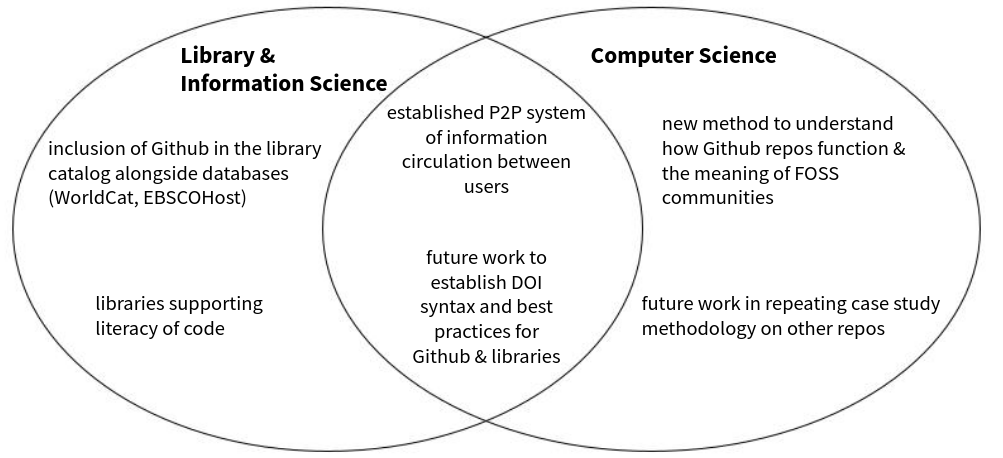
\includegraphics[width=.8\textwidth]{./images/results_venn.png}
\caption{"Venn Diagram to illustrate the outcomes for Library Science, Computer Science, and interdisciplinary outcomes."}
\vspace{0in}
\end{center}
\end{figure}

As a result of this thesis, it is possible and a valid analysis to apply concepts from Library and Information Science to understand the functionality of Github repositories, including the implementation of several new terms which describe the interdisciplinary connections in practical application. This outcome is significant for both Library and Information Science and Computer Science, as it opens the doors to further research. 

\section{Future Work}

Future work beyond this thesis includes repeating the pandas case study using the defined concepts and applying these to other repositories on Github, further study of centralized peer-to-peer systems and how this applies to version control systems, and determining the best practices for use and syntax of DOIs for Github and libraries. The completion of this case study also implies the practical use of approaching repositories in this way, for users of Github/Git, scholars studying the software, and students learning to use Github in a college undergraduate education environment. 

\subsection{Practical Application of Case Studies Methodology}

\subsubsection{Users of Github/Git}

The practical application of the CCAL and the case study methodology for users of Github gives meaning to use of this software, and understanding how the user experience can be best carried out. The decentralized nature of Github and the individual element of choosing to participate in contributing to/maintaining software complicates the practical application of these ideas because they must be communicated to the users. Because this is a specific method that maintainers are not aware of, the practical application would best be carried out by a more broad part of Github, such as Github Education and Github Docs. There is benefit to this being included in Github Education because it already instructs students of the program on how to contribute, so the methods could easily be incorporated in backing up why contributing in those ways are most beneficial. Including this information in the Github Docs may help more experienced users find this information, as they may be less inclined to work with Github Education. 

\subsubsection{Scholars}

For scholars, the case study and CCAL methodology extends into the field of Software Studies, which has been orginally defined by Marino \cite{marino2020critical} and contributed to by scholars such as Vee \cite{vee2017coding}. Although more focused on databases specifically, this also seems to include Ackermans' work \cite{ackermans2020appeal} because their approach to databases is also a critical reading of a software system. Because the CCAL and case study methodologies are interdisciplinary in nature, these systems in a scholarly environment may apply most to scholarship in interdisciplinary fields, such as Software Studies/Critical Code Studies and the Digital Humanities. Future work with these methodologies in a scholarly setting would involve re-applying the methods perhaps with further work in the specifics of reading the repository as a text, or the application of other humanities concepts to repositories alongside or in comparison to the methods defined in this thesis. 

\subsubsection{College Undergraduate Education}

A major component of teaching undergraduate computer science courses is the teaching of best practices for using Github. This covers several levels of computer science education, from learning to write descriptive commit messages in the earliest introductory classes to engaging with the issue discussion and pull request processes in software engineering classes. The methodology of the pandas case study and the actions within the CCAL methodology add meaning to the practical application of these best practises. If the meaning of the best practices were to be taught in addition to the best practices itself, students will have a complete understanding of the importance of best practices. This may lead students to be more inclined to follow best practices, as opposed to if the best practices are taught without the meaning behind them or a simplified meaning that they help with organization or communication alone. In reality, these best practices are upheld by a system that is understood by the methodology of this research. 



 
%----------------------------------------------------------------------------------------
%	BIBLIOGRAPHY
%----------------------------------------------------------------------------------------

\addtocontents{toc}{\vspace{2em}} % Add a gap in the Contents, for aesthetics
\unnumberedchapter{Bibliography} % Title of the unnumbered chapter
\bibliography{preamble/bibliography} % The references information are stored in the file named "bibliography.bib"


\end{document}  